%% The options are (you can only choose one from each group):
%%
%% 10pt, 11pt, 12pt: chooses the point size for the document. "11pt" is the
%%                   default.
%%
%% oneside, twoside: whether you want your document onesided or twosided. Note
%%                   that twosided is not guaranteed to work, and style
%%                   guidelines prohibit double sided printouts on final
%%                   copy. "oneside" is the default.
%%
%% draft, final: when printing drafts you can save a lot of paper by using the
%%               "draft" option. It switches to single spacing, displays overful
%%               hboxes with a black box, prints a version number on title page 
%%               and omits signature page. Of course for the final copy make
%%               sure to use the "final" option! "final" is the default.
%%
%% thesis, dissertation: switches between the style for a master's thesis and a 
%%                       Ph.D. dissertation. The differences are fairly minor
%%                       and limited to the front matter. "thesis" is the
%%                       default.
%%
%% actual, proposal: switches between actual document and proposal mode. In
%%                   proposal mode: the title page is simplified, the
%%                   version number is always printed, and the signature page
%%                   is omitted.
%%
%%% Load the new uhthesis document class
%\documentclass[11pt,final,dissertation,actual,subfigure]{uhthesis}
\documentclass[11pt,final,dissertation,actual,subfigure]{uhthesis}

%% hyperref package complains if this isn't here. Might be unneeded when
%% I switch to the new UH thesis style
%\paperheight = 11in

%% Switch to Times font
%\usepackage{times}
\renewcommand{\rmdefault}{ptm}

%%% Load some useful packages:
%% LaTeX2e graphics support
\usepackage{graphicx}
%%	using final option to force graphics to be included even in draft mode
%\usepackage[final]{graphicx}
%% Tell graphicx the default directory for all figures
\graphicspath{{figures/}}

%% Enable subfigure support
\usepackage{subfigure}

%% Provide longtable support, so tables can span multiple pages
\usepackage{longtable}

%% This is a patch of the original longtable package that I stumbled upon
%\usepackage{ltabptch}

%% Make pretty shaped paragraphs
\usepackage{shapepar}

%% Make subsubsections numbered and included in ToC
\setcounter{secnumdepth}{3}
\setcounter{tocdepth}{3}

%% Package to linebreak URLs in a sane manner.
\usepackage{url}

%% Define a new 'smallurl' style for the package that will use a smaller font.
\makeatletter
\def\url@smallurlstyle{%
  \@ifundefined{selectfont}{\def\UrlFont{\sf}}{\def\UrlFont{\small\ttfamily}}}
\makeatother
%% Now actually use the newly defined style.
\urlstyle{smallurl}

%% Define 'tinyurl' style for even smaller URLs (such as in tables)
\makeatletter
\def\url@tinyurlstyle{%
  \@ifundefined{selectfont}{\def\UrlFont{\sf}}{\def\UrlFont{\scriptsize\ttfamily}}}
\makeatother

%% Provides additional functionality for tabular environments
\usepackage{array}

%% Adds new functionality for tables
\usepackage{tabularx}

%% Create a variable width hrule. From:
%% http://tex.stackexchange.com/a/3447/22230
\makeatletter
\def\hlinewd#1{%
\noalign{\ifnum0=`}\fi\hrule \@height #1 %
\futurelet\reserved@a\@xhline}
\makeatother

%% Set up to create an index
%\usepackage{makeidx} 
%\makeindex

%% Puts space after macros, unless followed by punctuation
\usepackage{xspace}

%%% Personal macros
%% Hawai`i with okina
\newcommand{\Hawaii}{Hawai`i\xspace}
%% Hawai`ian with okina
\newcommand{\Hawaiian}{Hawai`ian\xspace}
%% Manoa with kahako
\newcommand{\Manoa}{M\=anoa\xspace}

%% Provides customization of lists
\usepackage{enumitem}

%% Now define question list type
\newlist{question}{enumerate}{1}
\setlist[question]{resume, label=\textbf{\arabic*.}}

%% Define multiple choice answer list type
\newlist{answer}{enumerate}{1}
\setlist[answer]{label=\alph*)}

%% Provides some useful symbols such as checkboxes, circles
\usepackage{wasysym}

%% Define checkbox answer list type
\newlist{checkbox}{itemize}{1}
\setlist[checkbox]{label=\Square}

%% Define radio button answer list type
\newlist{radiobutton}{itemize}{1}
\setlist[radiobutton]{label=\Circle}

%% Allows insertion of fixme notes for future work
%% Note, remove status=draft when printing final version!
\usepackage[footnote, nomargin, status=final]{fixme}
%\usepackage[footnote, nomargin, status=draft]{fixme}
%% turned off marginclue because it generates hbox overflows for each note :(
%\usepackage[footnote, nomargin, marginclue, status=draft]{fixme}

%%% Make URLs clickable
%% Colored links, best for reading PDF on computer
\usepackage[colorlinks, citecolor=blue, bookmarks=true]{hyperref}
%% Colored links and backreferences, for reading PDF on computer
%\usepackage[colorlinks, citecolor=blue, bookmarks=true, backref]{hyperref}
%% Turn off link coloring when printing black & white
%\usepackage[bookmarks=true]{hyperref}

%% Make \autoref from hyperref package capitalize things normally
\def\chapterautorefname{Chapter}
\def\sectionautorefname{Section}
\def\subsectionautorefname{Section}
\def\subsubsectionautorefname{Section}

%% Make links to captions point to the figure, not just the caption at bottom
\usepackage[all]{hypcap}

%% Set up to create a glossary
%\usepackage[toc]{glossaries}
%\makeglossaries

%% Since I'm using the LaTeX Makefile that uses dvips, I need this
%% package to make URLs break nicely
\usepackage{breakurl}

% correct bad hyphenation here
\hyphenation{strong-ly}

%% Useful if you just want to create a PDF of one include file
%\includeonly{appendix-actions}

%%% End of preamble
\begin{document}

%%% Declarations for Front Matter. Capitalize all of these values
%%% "normally". This allows the document class to format them properly.
%% Full title of thesis or dissertation, capitalized like a title should be.
\title{Software Trajectory Analysis: an empirically based method for automated software process discovery}
%% Your name, capitalized normally. Do not include any titles like Dr.
\author{Pavel Senin}
%% Month in which you intend to receive your degree (i.e. graduation).
%% Presumably this will be one of: May, August, or December.
\degreemonth{-}
%% Year of expected graduation.
\degreeyear{2013}
%% Type of degree to be conferred.
\degree{Doctor of Philosophy}
%% This is the chairperson of your committee. Do not use titles like Dr.
\chair{Philip M. Johnson}
%% The other members of your committee, seperated by "\\". Again, no titles,
%% and it is customary to list the outside committee member (if you have one)
%% last.
\othermembers{Kyungim Baek\\
Guylaine Poisson\\
Henri Casanova\\
Daniel Port}
%% The field in which you are obtaining your degree, capitalized normally.
\field{Computer Science}
%% 4-6 optional keywords/phrases for use in indexing or as search terms
%\keywords{software process, time series classification, data mining, knowledge discovery}

%% The version number of your document. Consistent use of this will enable you
%% to tell old drafts from new ones. Final actual documents omit this
%% automatically so you can use it without fear of submission problems at the
%% end. If you do not define this parameter, it defaults to "1.0.0".
\versionnum{1.0.0}

%%% Create the title page from all the information above. Note that the
%%% titlepage is outside the front matter.
\maketitle

\begin{frontmatter}

%%% Signature page is no longer included in the manuscript, Form IV replaces it

%%% Create the copyright page
\copyrightpage

%%% Bring in the dedication page from external file
%%%%%%%%%%%%%%%%%%%%%%%%%%%%%% -*- Mode: Latex -*- %%%%%%%%%%%%%%%%%%%%%%%%%%%%
%% thesis-dedication.tex -- 
%% Author          : Robert Brewer
%% Created On      : Fri Sep 25 14:33:09 1998
%% Last Modified By: Robert Brewer
%% Last Modified On: Thu Mar 16 12:03:14 2000
%% RCS: $Id: thesis-dedication.tex,v 1.3 2000/03/17 21:26:34 rbrewer Exp $
%%%%%%%%%%%%%%%%%%%%%%%%%%%%%%%%%%%%%%%%%%%%%%%%%%%%%%%%%%%%%%%%%%%%%%%%%%%%%%%
%%   Copyright (C) 1998 Robert Brewer
%%%%%%%%%%%%%%%%%%%%%%%%%%%%%%%%%%%%%%%%%%%%%%%%%%%%%%%%%%%%%%%%%%%%%%%%%%%%%%%
%% 

\begin{dedication}

%% Maybe a Kukui Cup logo outline?

  \null\vfil
  {\large
    \begin{center}
      \heartpar{To Yuka: thanks for all the love, support, and patience you
        have shown me while I worked on my Ph.D. It is most deeply appreciated.}
    \end{center}}
  \vfil\null

\end{dedication}


%%% Bring in the acknowledgements section from external file
\begin{acknowledgments}

Like any research project, this one could not have been completed without the help of a number of people. My thanks go to Prof. Philip Johnson, who has been my wonderful advisor and mentor for over 20 years. Thanks for going ``all in'' for sustainability: there are few advisors that decide to change their entire research program the way you did!
  
I'd like to thank my parents Bill and Ellen Brewer for their support both moral and professional.

I'd also like to thank past and present members of CSDL in chronological order: George Lee, Yongwen Xu, Michelle Kat\-chuck, and Carleton Moore. The Kukui Cup research project would not have happened without your long hours and hard work.

Actually running a Kukui Cup required an even bigger team. I'd like to thank Kaveh Abhari, Hana Bowers, Greg Burgess, Caterina Desiato, Risa Khamsi, Alex Young, and Chris Zorn for their work on the 2011 UH Kukui Cup. University of \Hawaii Student Housing was incredible in their financial and logistical support of the Kukui Cup from: Michael Kaptik, Michael Weakley, Shawn Patrick, Michiko Maggi, Randall Watanabe, and Roland Castillo.

Of course there would be little point in having a Kukui Cup Challenge if nobody participated. I'd like to thank all the residents who played the Kukui Cup; I hope you learned something of value.

I would like to thank my committee members Prof. Martha Crosby, Prof. Scott Robertson, Prof. Daniel Suthers, and Prof. Anthony Kuh for taking the time to read and evaluate this dissertation. In particular, Scott was generous with his time in helping me with questionnaire data analysis.

Several researchers from outside the University of \Hawaii have provided valuable feedback on the Kukui Cup, including Tawanna Dillahunt, Nicole Sintov, Prof. Jon Froehlich, Prof. Eric Paulos, Prof. Sam Joseph, Jim Cummings, and Dante Anderson.

This research is supported in part by grant IIS-1017126 from the National Science Foundation; the HEI Charitable Foundation; the Hawaiian Electric Company; and the State of Hawaii Department of Business, Economic Development and Tourism. We are also thankful for the support from the following organizations at the University of Hawai`i: Facilities Management, and the Department of Information and Computer Sciences. 

Funding from the Center for Renewable Energy and Island Sustainability (REIS) was essential to getting this research project off the ground. REIS has personally supported me with a research assistantship over the course of my work on the Kukui Cup, and provided initial seed funding before we obtained other grants. I've also appreciated the opportunity to interact with other students and faculty from REIS, which has exposed me to other perspectives on this research area.

Last but not least, I thank Yuka Nagashima, the love of my life, for all that she has done in support of me. You were a sounding board for my ideas, you always had insightful comments on the paper drafts you volunteered to read, and you even helped out with Kukui Cup events on your birthday. I could not have done it without you. Mahalo.

\end{acknowledgments}


%%% Bring in the abstract section from external file
%%%%%%%%%%%%%%%%%%%%%%%%%%%%%% -*- Mode: Latex -*- %%%%%%%%%%%%%%%%%%%%%%%%%%%%
%% abstract.tex -- 
%% Author          : Joseph Dane
%% Created On      : Fri Oct  8 21:04:34 1999
%% Last Modified By: Joe Dane
%% Last Modified On: Wed Oct 20 12:15:34 1999
%% RCS: $Id$
%%%%%%%%%%%%%%%%%%%%%%%%%%%%%%%%%%%%%%%%%%%%%%%%%%%%%%%%%%%%%%%%%%%%%%%%%%%%%%%
%% Copyright (c) 1999 Joseph Dane
%%%%%%%%%%%%%%%%%%%%%%%%%%%%%%%%%%%%%%%%%%%%%%%%%%%%%%%%%%%%%%%%%%%%%%%%%%%%%%%
%% 

\begin{abstract}

  Effective program size measurement is difficult to accomplish.  Factors
  such as program implementation language, programmer experience and
  application domain influence the effectiveness of particular size metrics
  to such a degree that it is unlikely that any single size metric will be
  appropriate for all applications. This thesis introduces a tool, LOCC,
  which provides a generic architecture and interface to the production and
  use of different size metrics.  Developers can use the size metrics
  distributed with LOCC or can design their own metrics, which can be
  easily incorporated into LOCC.  LOCC pays particular attention to the
  problem of supporting incremental development, where a work product is
  not created all at once but rather through a sequence of small changes
  applied to previously developed programs.  LOCC requires that developers
  of new size metrics support this approach by providing a means of
  comparing two versions of a program.  LOCC's effectiveness was evaluated
  by using it to count over 50,000 lines of Java code, by soliciting
  responses to a questionnaire sent to users, and by personal reflection on
  the process of using and extending it.  The evaluation revealed that
  users of LOCC found that it assisted them in their development process,
  although there were some improvements which could be made.


\end{abstract}


%%% Generate list of FiXmes, will be silent in final mode
\listoffixmes

%%% Generate table of contents
\tableofcontents

%%% Generate list of tables
\listoftables

%%% Generate list of figures
\listoffigures


\end{frontmatter}

%%% Include each chapter
% my main text chapters
\chapter{Introduction}
Delivering high quality software products within the budget and in time is the main goal and the most 
challenging task of Software Engineering. Years of scientific research in this area resulted in a 
number of software processes providing detailed guidelines on how to reach 
the goal efficiently. These processes manifested themselfs as the means for improvements in terms 
of quality, speed and cost over existing practices. Many were implemented and tested within academic 
and industrial settings and proved proposed superiority. Some of these processes were successfully 
adopted and standardized in industry shaping the best practices of contemporary software development 
\cite{citeulike:9962021}. Moreover, there are plethora of processes for improving existing processes 
of software development on the team \cite{citeulike:9962027} and personal 
levels \cite{citeulike:9962022}.

The processes I am mentioning here are the well-known large formal models such as Waterfall and Spiral, 
as well as more flexible iterative agile approaches like XP, SCRUM or FDD. These are also sets of 
rules and recommendations which can be applied to certain stages of the software processes 
such as Test Driven Development or Pair Programming; there are general guidelines helping 
to improve the correctness of a product and standards, like CMMI or ISO 9000; guidlines for testing 
and measurements, code syntax rules and formatting styles, code comments 
recomendations \cite{citeulike:900855}. 

From the first sight, taking all this in account,  one would guess that 
the area of software processes is thoroughly explored and there are clear choices of processes 
and models for the one in charge making decision... But it is not true - despite many choices 
one can make, no one can foretell what is the ``best'' process to choose for certain constraints.
What managers are left with are the equal alternatives and vague promises. 
This deficiency in knowledge is the main coause of the ``software crisis'' phenomena point is supported by the fact that according to ``Chaos Report'' from the Standish 
Group (Rubinstein) \cite{SDTimes} only ``35\% of software projects in 2006 can be categorized as successful - meaning 
they were completed on time, on budget and met user requirements''. 
These thirty five percent of success clearly saying that it is somewhat difficult to make 
a statement that we are fully understand and able to control software processes. 
Moreover, over years, while this idea of a software process formalizations shaped the 
programming practices, which once thought to be a creative human activity accessible by amateurs 
and hobbyists \cite{citeulike:9958822} into a serious engineering discipline, bounded 
by requirements for education, standardized processes, rules, certifications, and strict 
financial requirements from stakeholders the opposite idea was born - the idea of 
software development as a craft. Interesting that such a duality of views can be found 
in the work of a single person \cite{citeulike:5203446}.

Clearly, there is a great room for research and improvement of our understanding of software processes.
This exploratory study is yet another attempt at the understanding. In my research work I am 
exploring techniques aiming the understanding of small processes which are 
rather the reflection of personal behaviors or habits of software development rather than a 
formalized constructs. Also, I would like to emphasize, that in this work I will not 
address the need and means of the process synthesis, its quality assessment, productiveness
or any topics related to the software product itself; I would rather focus on the specific issue - 
uncovering an existence and studying the programming habits. 

This thesis presents a methodology for finding recurrent behaviors through the 
analysis of the variety of software process artifacts left after performing a 
software process. I have called this methodology ``Software Trajectory'' and it consists 
of four distinct steps. Each of these steps has a specific goal and compromising variety of 
means to reach it. 
At first software process artifacts are identified and collected. 
At second, they are cleaned, organized and classified. 
On the third step particular research questions are formulated and data are organized and indexed. 
And finally, a set of KDD techniques is applied in order to undercover recurrent behaviors which 
could potentially shed a light on the performed process details. 

My personal motivation for performing this work is coming from the recognition of the 
importance of the software in our lives and the severity of issues with its development. 
Through my everyday experiences with software development and use I have stumble upon 
a number of issues which made me realize that mentioned ``software crisis'' phenomena is very real.
As a user in industrial and academic settings I often find myself facing software failures 
which create numerous difficulties for reaching production or research goals. As a developer, 
in an attempt to be productive and in order to deliver a better software I have studied and 
explored a number of formal processes, however, sometime I found myself seeing a very little of 
rationale behind their application, and moreover, in this exploration, when facing the process
application failing to help I was unable to comprehend what exactly went wrong and what need 
to be changed. All of these experiences made me studying software process research and exploring
novel approaches to software process recovery on my own in order to understand software process better.

\section{Research area overview}
As mentioned above, in this thesis I am focusing on a very narrow subject - exploring approaches
for uncovering of recurrent behaviors or ``programming habits'' out of software process artifacts.
Before narrowing further 


Software is usually coded by teams. Members of these teams are agreed and bound to use 
a particular technologies and development tools, they also agree on following well defined 
development process which is constrained by a timeline and budget. These are necessary 
constraints to keep work organized, however there is a great freedom in what they actually 
do in every single moment of time in order to progress towards lines of code which eventually 
will result in software. For example one developer may follow test first process while
another writes tests at last.  This freedom of choice in ordering of development activities 
while being much appreciated by talented and creative individuals creates an impression 
of chaotic and unordered activities for random observers, newbies and people in 
charge - so there we have all the attempts of imposing an order 
(or control) on all of the development activities. Metrics and models of processes





%
%\section{Research problem statement and Scope of the dissertation}
Software is coded by humans. Whether in team or individually, humans perform relevant 
daily activities in order to reach the goal - deliver the software. Understanding of these
human activities spanning through the life-cycle of the software, in connection with personal 
and team's motivations, environment settings and constraints essentially enables one to
comprehend the software process. It is worth noting, that roughly \todo[inline]{put here something 
about two components - the human-driven, non-recurrent and creative activity - 
the behavioral component - and the process and the technology/toolkit component which
provides a measurable marginal effect}

\todo[inline]{Here, put stuff about observing the process and artifacts availability}

\todo[inline]{Here, put stuff about time-series analysis flexibility and its difference from 
convenient process mining.}

While it is shown by the large body of previous research, that it is technically possible 
to factor out the impact of the technology and the process, the impact of the behavioral 
component is yet to be studied. Hence, my primary research question is this:
\begin{myindentpar}{0.07\linewidth}
 \textbf{Can we discover recurrent behaviors in software processes from project
  repository artifacts?}
\end{myindentpar}

Obviously, in order to answer this question correctly two interconnected, secondary, question must be resolved:
\begin{myindentpar}{0.07\linewidth}
 \textbf{Which kind of software process artifacts reflect recurrent behaviors?}
\end{myindentpar}
\begin{myindentpar}{0.07\linewidth}
 \textbf{Which data-mining method is sensitive and selective enough to recover recurrent behaviors
from software process artifacts?}
\end{myindentpar}
These two can be broken down further to the problem of studying and classifying of software process artifacts,
methods of their extraction and partitioning, and, of course, the problem of recurrent behaviors discovery.

As was mentioned above, in this thesis I am focusing on a very narrow subject - exploring approaches
for uncovering of recurrent behaviors or ``programming habits'' out of software process artifacts.
While I will show, that, potentially, many software-development activity behaviors can be recovered,
their classification, impact and performance studies are beyond the scope of this thesis.


%
%\section{Organization of the dissertation}
%
\chapter{Prior and related work}\label{chapter_background_work}
My research focuses on the techniques which aide in the knowledge discovery from a process of 
software development. There is much previous relevant work related to my goal processes; work combines is based on previous research from multiple research areas: software engineering, 
software repository mining, process mining, knowledge discovery from time series,
and information retrieval. 

By extending existing knowldge about software processes and repository mining and combining 
it with a novel technique for knowledge discovery from time series, 
I was able to develop an automated framework for recurrent behaviors discovery from publicly 
available software repositories.

In this chapter I will review previous work relevant to my research.

\section{Engineering in software development}
Since the invention of Charles Babbage’s difference engine in 1822, computers (hardware) 
have required a means of instructing them to perform a specific task. This means is known 
as a programming language. By using programming instructions, software develeopers (programmers)
write the software that is collections of computer data and instructions, which is used by 
users to accomplish specific tasks. The very first software, or more precisely a set of 
instructions implementing a method for calculating a sequence of Bernoulli numbers using 
Charles Babbage's Analytical Engine, was designed by Ada Lovelace in 1942 and predates modern 
computers. 

As time has progressed, computers have made giant leaps in processing power and become 
general-purpose computing devices. Consequently, the variety of software and 
the complexity of its development has grown ``several orders of magnitude'' \cite{naur_crisis_68}. 
This effectively created a number of organizational problems which dominated development of 
early software systems. Among these, historians are mentioning increasing scale of software projects, 
excessive ambition, difficulties in estimating project cost and length, inadequate documentation, 
skimping on design and testing \cite{mahoney_roots_1990} \cite{citeulike:12748733} 
\cite{citeulike:833903}.

All these problems were recognized at the NATO Conference on Software Engineering, held in Garmisch,
Germany in 1968. It worth noting, that before the actual conference, as was pointed by the 
conference proceedings editors, engineering paradigm was chosen without actual plan of actions - 
\textit{``the phrase ``software engineering'' was deliberately chosen as being provocative, in implying 
the need for software manufacture to be [based] on the types of theoretical foundations and practical 
disciplines[,] that are traditional in the established branches of engineering''} \cite{citeulike:12787786}.
At the conference, it was acknowledged, that the increasing complexity of programming 
work had overwhelmed the technical and managerial ability of software teams: software was shipped late,
over budget, worked inefficiently, and was unreliable. Later, while working on the proceedings, the term 
``software crisis'' was coined by the editors in order to describe the desperate state of 
software development and its increasing complexity \cite{naur_crisis_68}.

Nevertheless, the ``software engineering'' idea was provocative enough to shape the minds of researchers 
and practitioners. At large, it was accepted that the software can be successfully ``manufactured'' 
through ``engineering'' - i.e. with the application of a systematic, disciplined, quantifiable approach 
to the design, development, operation, and maintenance. 

Using this paradigm, researchers and practitioners designed a number of software development processes 
providing detailed guidelines on how to reach the goal - deliver the software - efficiently and in time. 
These processes were declared as the means for improvements in terms of quality, speed, and execution cost 
over existing practices. They were studied within academic settings and adopted by industry. 
Some of this processes were further standardized, shaping the best practices of contemporary 
software development \cite{citeulike:9962021}. 

The processes, that I am addressing here, can be found in numerous studies and described at length 
in industrial and academic literature. Too numerous to name, they can be categorized by the level 
of their application:
\begin{itemize}
 \item global organizational standards, like CMMI, ISO 9000, and SPICE. 
 \item large industrial software models, such as Waterfall, Spiral, Cleanroom, etc.
 \item smaller scale, flexible methodologies: FDD, TDD, Pair Programming, etc.
 \item general guidelines and principles aiming to improve the software process flow, 
such as ``build before commit'' and others.
 \item and finally, the processes for improving existing processes of software development 
on the organizational, team, and personal levels: TSP, PSP, Six Sigma, etc.
\end{itemize}
While some of these are products of a ``technology transfer'' - resulted by direct copying or by an 
application of existing engineering principles to software development process (like Waterfall model), 
some, and in particular agile methods, considered to be particular to software-engineering. 

\subsection{Issues with engineering-like processes}
Currently, in Software Engineering, there are numerous software process, models, methodologies, 
and coding conventions exist for any level and any stage of the software development carried out by 
any team size at any project scale. 
This amount of well-grounded and documented knowledge creates an impression, that the area of 
software development process is thoroughly explored, and that there exists a deterministic choice 
for a model and a processes for any given software project leaving almost no doubts in 
its faith - it will be completed according to the specification, in time, and under the budget.

However, it is far from being true - software projects do fail at the considerably high rate and 
many challenges exist in software product development. Many software projects continue to run over 
the budget, do not meet the schedule. Some of the seemingly proper executed projects caused property 
damage \cite{citeulike:11044022}, and a few projects caused loss of life \cite{citeulike:712058}. 
The ``Chaos Report'' from the Standish Group, that only ``35\% of software projects in 2006 can be 
categorized as successful - meaning they were completed on time, on budget and met 
user requirements'' \cite{chaos2006}. These thirty two percent of success clearly manifest that 
it is somewhat illusory statement that we are capable to understand and to control software processes.

This rather poor performance of the mainstream software engineering processes 
ignited a new wave of research in the field in recent decades. Gradually, researchers and 
practitioners alike recognized, that a direct application of classical engineering - that 
excludes a ``human component'' by governing software processes in a top-down fashion 
might be somewhat erroneous. 
Also, it was recognized that over many years, continuous formalization of the field and 
excessive attention to software process metrics may malformed not only the software development 
practices landscape, but education and a professional code of conduct. 
This recognition forced some of the professional associations to review their licensing policies 
\cite{citeulike:11045517} and some educators to change their opinions \cite{citeulike:5203446}. 

\section{Alternative software processes}
In parallel with industrial engineering-like software processes, another phenomena, 
the Free/Libre Open Source Software (FLOSS) development arose and proven its efficiency and effectiveness.
The FLOSS processes are significantly different from typical SE process on many levels:
\begin{itemize}
 \item First of all, FLOSS processes are highly geographically distributed, which significantly contradicts 
 to developers collocation usually assumed by the most of the SE processes. 
 \item Secondly, open-source processes do not explicitly define timeline, developers roles, and 
 the process itself. Typically, the project flow is rarely governed and does not require any sort of 
 documented software process. Most of FLOSS projects accept for review and embed source code from anyone.
 \item Finally, FLOSS delivers software free of charge, promoting its reuse, modification, and redistribution.
 However, mostly due to this, the maintenance and the support are rarely provided.
\end{itemize}

Nevertheless, despite to the apparent lack of the control over the software processes in FLOSS projects, they 
has proven their ability to deliver large in size software systems of high quality for the fraction of cost 
of similar industrial projects.

Most of the success is contributed to the motivation of open source developers.

Lately, third approach to software development emerged - software craftsmanship emerged 
\cite{citeulike:11058561}, \cite{citeulike:11058554}. The followers of this methodology 
are not only focused on the delivering ``well crafted'' software and continuously adding value,
but on the apprenticeship - on forming communities and engaging more people in software development.
While recommendation exists \cite{citeulike:11058784}, little known about the research 
in software craftsmanship and apprenticeship processes.

All this continues to engage thoughts and fuels the search not just for the exact definition 
of software development, but deep, fundamental for efficient processes resolving. 
Is software development an engineering discipline? Is it a craft \cite{citeulike:5203446}? 
Or is it an art \cite{citeulike:11045694}?

Answers to these questions would require extensive interdisciplinary studies to be made, 
but what is obviously clear, is that formal software development process, as an engineering 
is a creative, human activity. 
Whether software is coded 
by team where its members have a variety of skills and experience, or by a single individual,
they all driven by their believes and motivations. While usually developers agree on the use of 
particular technologies, development tools, and a development process with imposed timeline and 
a budget, the software process is - as many other human activities - highly creative and mostly 
non-recurring. Thus, the choice of methodology, technology, or tools provides only a marginal 
effect on this human-based and human-driven process. While this effect can be measured through 
the common approach by using a control environment factoring out human component, the most of 
the difference, which lies in human creativity, motivation and productivity is unknown and yet, 
mostly immeasurable.

\section{Process discovery}\label{process.discovery} 
Process is a general term describing a phenomenon unfolding in time and has a variety of meaning depending
on the field. While in this thesis I focus on a particular kind - software processes, moreover, on the particular process 
building block - recurrent behaviors, in this section I outline few general conceps and previous research work that 
was applied to software processes.

\subsection{Stochastic process}
In probability theory a stochastic (or a random) process denotes a collection of random variables which typically used
to represent the evolution of some random value or a non-deterministic system in time. The specificity of a stochastic 
process is that while its initial condition is known, it can evolve in infinitely many directions. 
In the simple case of discrete time, a stochastic process amounts to a sequence of random variables usually known as 
a stochastic time series. 
The examples of stochastic time series include signals such as speech, audio and video, medical data such as a 
patient's EKG, blood pressure or temperature, stock market and exchange rate fluctuations, and random movement 
such as Brownian motion or random walks.

The common approach to stochastic processes treats them as functions of one or several deterministic arguments whose 
values are random variables that taken from parametrized probability distributions. For example the growth of a software 
project size can be modeled by its relationship with time and effort as was shown by numerous research work 
\cite{citeulike:330266} \cite{citeulike:12849755} \cite{citeulike:12849753} \cite{citeulike:328047} \cite{citeulike:12849771}
which suggests that the evolution of various software metrics can be modeled with Double Pareto distribution.

While stochastic process is useful for predicting of what likely to be observed, they usually are too low level to be used for
a software process modeling. For example a variety of development events such as maintenance, correction, new function,
and enhancement may cause change in a number of source code files and lines, but in order to discover these events 
from the metrics changes an additional mapping procedure, such as coding performed by human experts or classification 
with automated techiques is required. Once mapping is applied, a number of tools and techniques usually called ``business 
intelligence tools'' can be applied to these collections of events.

Although process mining in the business domain is a well-established field with much software developed up to date 
(ERP, WFM and other systems), ``Business Process Intelligence'' (BPI) tools usually do not perform process discovery and 
typically offer relatively simple domain-oriented analyses that depend upon a correct a-priori process model 
\cite{citeulike:3718014} \cite{citeulike:5044991}. 
This fact restricts off-shelf application of business domain process mining techniques to software engineering, where 
processes are usually performed concurrently by many agents, are more complex and typically have a higher level of noise. 
Taking this fact in account, I will review only the approaches to stochastic process mining for which applicability to software 
process mining was expressed. 

In particular I review four approaches in the rest of this section: 
\begin{itemize}
 \item the work by Cook \& Wolf in that discuss an event-based framework for process discovery based on grammar 
  inference and finite state machines. 
  The authors directly applied their framework to Software Configuration Management (SCM) logs demonstrating satisfactory 
  results \cite{citeulike:328044}.
 \item the work by Van der Aalst et al. where they demonstrate the applicability of Transition Systems and labeled Petri nets 
  to process discovery in general \cite{citeulike:3718014} and the subsequent work by van der Aalst and Rubin 
  that discusses software process mining \cite{citeulike:1885717}.
 \item the approach by Jensen \& Scacchi \cite{citeulike:5043664} that describes a framework built upon an universal generic 
  meta-model and specific to the observed processes models which are iteratively built and revised during case studies. 
  The particular value of this work is in the demonstration of the importance of the correct mapping between process artifacts 
  and process entities as well as a demonstration of iterative process revision that emphasizes the importance of pre-existing 
  domain knowledge in the effective pruning of the search space.
\item the recent work by Hindle et al. \cite{citeulike:9114115} \cite{citeulike:9007622} that shows the possibilty of software 
  process evidence discovery from software process artifacts.
\end{itemize}

Notice, that all reviewed approaches require a mapping to be provided. In addition all reviewed approaches have difficulties 
dealing with concurrency, which, in turn, is inevitable in the software process usually performed by many agents. 
Much successive work has been done extending reviewed approaches to the concurrent processes. 
%Among others, Weijters \& van der Aalst in \cite{citeulike:5128101} propose heuristics to handle concurrency and noise issues, 
%while van der Aalst et al. in \cite{citeulike:5128110} discuss a genetic programming application. 

\subsection{Process discovery through Grammar Inference} \label{grammar}
One of the pioneering process discovery techniques was developed by Cook \& Wolf in \cite{citeulike:328044}. The authors 
developed a generic techniques intended to discover process models from event streams. The authors did not really intend to 
generate a complete model, but rather to generate sub-models that express the most frequent patterns in the event stream.
They designed a framework which collects process data from ongoing software process or from history logs, and generates a 
set of recurring patterns of behavior characterizing observed process. In their work they extended two methods of 
\textit{grammar inference} from previous work: purely statistical (neural network based \textit{RNet}) and purely algorithmic 
(\textit{KTail}) as well as developed their own Markovian method (\textit{Markov}). 

\textit{Process discovery}, in the author's opinion, resembles the process of \textit{grammar inference}, which can be defined 
as the process of inferring a language grammar from the given set (sample) of sentences in this language. 
In the demonstrated approach, words of the language are atomic events of the dynamic process, whether sentences built from 
such words, are describing the behavior of a process. 
Consequently, the inferred grammar of that language is the formal model of the process. Cook \& Wolf expressed such grammars 
as Finite State Machines (FSMs) and implemented a software tool for the mining of the software process. 
This tool was successfully tested in an industrial case study.

\begin{figure}[tbp]
   \centering
   \includegraphics[width=140mm]{inference.eps}
   \caption{Process discovery through the grammar inference: panel a) a sample event stream (simple process involving three 
   types of events: Edit, Review, and Checkin); and FNA results obtained by applying three methods of process discovery from 
   Cook \& Wolf \cite{citeulike:328044}.}
   \label{fig:inference}
\end{figure}

The first method extended by the authors, the neural-network based grammar inference, RNet algorithm, defines a recurrent 
neural network architecture which is trained by the sequences of events. After training, this neural net is able to characterize a 
current system state by looking on past behavior. The authors extract the FSM from the trained neural network by presenting 
different strings to it and extracting the hidden neurons activity through observations. Due to the nature of Neural Net, closely 
related activation patterns are clustered into the same state; therefore, by noting the current pattern, the input token, and the 
next activation pattern, transitions are recorded and compiled into the inferred FSM.

The second method investigated, is a purely algorithmic KTail method, which was taken from the work of 
Biermann \& Feldman \cite{citeulike:5120603}. The idea is that a current state is defined by what future behaviors can occur 
from it. The \textit{future} is defined as the set of next $k$ tokens. By looking at a window of successor events, the KTail 
algorithm can build the equivalence classes that compose the process model. The authors extensively modified the original 
KTail algorithm improving the folding in the mined model making to make it more robust to noise.

The Markov based method developed by the authors is based on both algorithmic and statistical approaches. 
It takes to account past and future system behavior in order to guess the current system state. Assuming that a finite number 
of states can define the process, and that the probability of the next state is based only on the current state (Markov property), 
the authors built a $n^{th}$-order Markov model using the first and second order probabilities. Once built, the transition 
probability table corresponding to the Markov model is converted into FSM which is in turn reduced based on the user-specified 
cut-off threshold for probabilities.

The authors implemented all three of these algorithms in a software tool called \textsc{DaGama} as a plugin for larger software
system called Balboa \cite{citeulike:5120757}. By performing benchmarking, Cook \& Wolf found that the Markov algorithm was 
superior to the two others. RNet was found to be the worst of the three algorithms. 

Overall, while having some issues with the complexity of produced output and noise handling, the authors proved applicability 
of implemented algorithms to real-world process data by demonstrating an abstraction of the actual process executions and 
capturing important properties of the process behavior. The major backdraw of the approach, as stated by the authors, 
lies in the inability of the FSMs to model concurrency of processes which limits its applicability to the software development process.
Later, they addressed this limitation \cite{citeulike:5128143}.


\subsection{Incremental Workflow Mining with Petri Nets}
Another set of findings relevant to my research approach was developed by Rubin
et al. \cite{citeulike:1885717} and van der Aalst et al.
\cite{citeulike:3718014} and is called \textit{incremental workflow mining}. The
authors not only designed sophisticated algorithms but built a software system
using a business process mining framework called ProM by van Dongen et al.
\cite{citeulike:5043673} which synthesizes a Petri Net corresponding to the
observed process. The system was tested on SCM logs and while the process
artifacts retrieved from the SCM system are rather high-level, the approach
discussed is very promising for the modeling of software processes from the
low-level product and process data.

\begin{figure}[tbp]
   \centering
   \includegraphics[height=65mm]{petri.eps}
   \caption{Illustration of the ``Generation and Synthesis Approach'' from
\cite{citeulike:5043673}: a) Transition System with regions shown; b),c) Petri
Nets synthesized from the Transition System.}
   \label{fig:petri}
\end{figure}

Within the incremental workflow mining framework, the input data from the SCM
audit trail information is mapped to the event chain which corresponds to the
software process artifacts. The authors call this process \textit{abstraction on
the log level} which is implemented as a set of filters which not only
aggregates basic events into single high-level entities but also removes data
irrelevant to the mining process (noise). 

The event chain constructed through the abstraction is then treated with the
\textit{Generate} part of the \textit{``Generate and Synthesis''}
\cite{citeulike:3718014} algorithm in order to generate a \textit{Transition
System} which represents an ordered series of events. This algorithm looks at
the history (prefix) and the future (suffix) sequences of events related to the
current one in order to discover transitions.  When applied to the abstracted
log information, the algorithm generates a rather large Transition System graph
where edges connect to abstracted events. This transition system is then
successively simplified by using various reduction strategies such as ``Kill
Loops'', ``Extend'', ``Merge by Output'' and others; it is possible to combine
these reduction strategies in order to achieve a greater simplification.

At the last step of the incremental workflow mining approach, Transition Systems
are used to \textit{Synthesize} labeled Petri nets (where different transition
can refer to the same event) with the help of \textit{``regions theory''}
\cite{citeulike:5128170}. As with the Transition System generation, the authors
investigate many different strategies of Petri nets synthesis, showing
significant variability in the results achieved. (see Figure \ref{fig:petri}).

The significant contribution of this research is in the generality of the
method. It was shown that by tuning the ``Generate'' and ``Synthesize'' phases
it is possible to tailor the algorithm to a wide variety of processes. In
particular, as mentioned before, Rubin et al. successfully applied this
framework to the SCM logs analysis.

\subsection{Reference model for Open Source Software Processes Discovery}
Jensen \& Scacchi in \cite{citeulike:5043664} take a somewhat different approach from the previously discussed research efforts. The authors are follow a top-down approach and do not try to build a software process model from available process artifacts. Instead, they try to develop a software process \textit{reference model} by iteratively refining mapping between observed artifacts and the model entities. 

The proposed software process \textit{reference model} is a layer which provides a mapping from the underlying recognized software process artifacts into a higher level software-process meta-model by Mi \& Sacchi \cite{citeulike:5128872}. The iterative revision of the reference model vocabulary of mapped terms (Figure \ref{fig:refterm}) is performed through case studies. During such a study, the observed process artifacts such as SCM logs, defect reports and others are queried with terms from the reference model pulling correlated artifacts which are revised and curated by the process expert and lead to the further revisions of the terms taxonomy on the next iteration.

\begin{figure}[tbp]
   \centering
   \includegraphics[height=35mm]{refterm.eps}
   \caption{Example of the reference model mapping from \cite{citeulike:5043664}.}
   \label{fig:refterm}
\end{figure}

In the relation to my research, I am envisioning the application of such iterative ``meta-model driven approach'' for characterization of the discovered recurrent patterns with unknown generative phenomena. The creation of the low-level recurrent patterns taxonomy through successive mapping into the meta-model assures from a ``nonsense patterns'' discovery.

\section{Mining software repositories}
However, in these and other research work based on mining of software process artifacts it was shown, 
that while public availability of artifacts is minimizing observability and privacy issues, the nature 
of these artifacts creates a number of other challenges, which limit the possible scope of the research 
and significantly elevate the complexity of the process discovery:
\begin{itemize}
\item First of all, the artifacts are created by developers and users not in order to enable the research,
but merely to support software development activities. Thus, the process-related information content of these
artifacts is questionable.
\item Secondly, the majority of these artifacts (change records, defect reports, assigned tasks, etc) 
typically represent a snapshot of the software project state rather than reflect any of performed actions, 
thus it might be simply impossible to infer any of completed software development events \cite{citeulike:1296888}.
This fact effectively renders obsolete a majority of previously developed event-based process discovery tools.
\item Thirdly, developers and users not only create and submit to repositories artifacts on their own volition,
but most of the change management system (such as Git, Subversion, and Gerrit) offer an asynchronous workflow, 
where the locally created artifacts might never be committed \cite{citeulike:2280690} \cite{citeulike:9037939}. 
Therefore, artifacts are displaced in time and it is often impossible to know exactly when their content was created.
\item Finally, the high volume of produced artifacts and their dimensionality demands for automated, high throughput 
techniques robust to the noise \cite{citeulike:12550438}, \cite{citeulike:7853299}, \cite{citeulike:4534888}.
\end{itemize}

While many behaviors are simply not observable through artifacts because they are never recorded
and do not leave any quantifiable evidence behind, for example phone-calls, face-to-face meetings, and 
private communications. 

\section{Knowledge discovery in time series}

%
%\chapter{Research method}

\section{Software process artifacts}
\subsection{Artifacts availablility}
\subsection{Artifacts extraction}

\section{Software process activities}
\subsection{Activities reconstruction}
\subsection{Activities partitioning}

\section{Recurrent activities mining}

\section{Software Trajectory - an approach}


%
%\chapter{Case Studies}

\input{case_eclipse}

%
%\chapter{Conclusions}
The ultimate premise of STA is to provide means for empirical guidance of developers and project 
management in software process execution and decision-making improvement.



%%% Switch to appendix mode
\appendix
%%% Bring in any appendices from external files
%\chapter{Publication List}
\label{app:publication-list}

These are the publications that have come out of this research that I have authored or co-authored:

\section{Journal Paper}

\begin{itemize}

\item Robert S. Brewer, \textbf{Yongwen Xu}, George E. Lee, Michelle Katchuck, Carleton A. Moore, Philip M. Johnson. Three Principles for the Design of Energy Feedback Visualizations. In   
\emph{International Journal On Advances in Intelligent Systems}, Vol. 3 \& 4, No. 6. (2013), pp. 188-198

\end{itemize}

\section{Conference Papers}

\begin{itemize}

\item \textbf{Yongwen Xu}, Philip M. Johnson, George E. Lee, Carleton A. Moore, Robert S. Brewer. Makahiki: An open source serious game framework for sustainability education and conservation.   
In \emph{Proceedings of the 2014 International Conference on Sustainability, Technology, and Education (STE 2014)}, Taiwan, December 2014
 	
\item \textbf{Yongwen Xu}, Philip M. Johnson, Carleton A. Moore, Robert S. Brewer, Jordan Takayama. SGSEAM: Assessing serious game frameworks from a stakeholder experience perspective.   
In \emph{Proceedings of the First International Conference on Gameful Design, Research, and Applications (Gamification 2013)}, Ontario, Canada, October 2013

\item Robert S. Brewer, \textbf{Yongwen Xu}, George E. Lee, Michelle Katchuck, Carleton A. Moore, and Philip M. Johnson. Energy feedback for smart grid consumers: Lessons learned from the Kukui Cup. In \emph{Proceedings of the Third International Conference on Smart Grids, Green Communications and IT Energy-aware Technologies (ENERGY 2013)}, Lisbon, Portugal, 

March 2013.

\item Philip M. Johnson, \textbf{Yongwen Xu}, Robert S. Brewer, Carleton A. Moore, George E. Lee, and Andrea Connell. Makahiki+WattDepot: An open source software stack for next generation energy research and education. In \emph{Proceedings of the 2013 Conference on Information and Communication Technologies for Sustainability (ICT4S)}, Zurich, Switzerland, February 2013.

\item Philip M. Johnson, \textbf{Yongwen Xu}, Robert S. Brewer, George E. Lee, Michelle Katchuck, and Carleton A. Moore. Beyond kWh: Myths and fixes for energy competition game design. In \emph{Proceedings of Meaningful Play 2012}, October 2012.

\end{itemize}


\section{Workshop}

\begin{itemize}

\item Robert S. Brewer, George E. Lee, \textbf{Yongwen Xu}, Caterina Desiato, Michelle Katchuck, and Philip M. Johnson. Lights Off. Game On. The Kukui Cup: A dorm energy competition. In \emph{Proceedings of the CHI 2011 Workshop on Gamification}, Vancouver, Canada, May 2011.

\item \textbf{Yongwen Xu}. Designing a Serious Game Framework for Sustainability. In \emph{PhD Student  Workshop on ICT4S 2013}, Zurich, Switzerland, February 2013.

\end{itemize}

\section{Poster}

\begin{itemize}

\item  Robert S. Brewer, Philip M. Johnson, Michelle Katchuck, George E. Lee, \textbf{Yongwen Xu}. Lights Off. Game On. The 2011 Kukui Cup. In \emph{The Behavior, Energy and Climate Change Conference (BECC) 2011}, Washington DC, November 2011.

\end{itemize}


%\chapter{Physical Concepts: Power and Energy}
\label{app:power-energy}

When discussing energy, and in particular electricity, it is important to understand what power and energy are, and how they interrelate.

\section{Energy}

Energy is defined as the amount of work that can be done by a force. Most of us have an intuitive notion of energy: is makes things move, it heats things up, etc. There are many units used to measure energy: joules (a very small amount of energy), BTUs, calories. When talking about electricity, the most common unit is the watt hour, abbreviated as "Wh", which is equal to 3600 joules. A watt hour is the amount of energy required to to provide 1 watt of power for one hour. Note that from a certain perspective it is somewhat peculiar to measure energy in units that include power (watt), since power is defined in terms of energy in the first place. This underlines how central the concept of power is in most of our dealings with electricity.

\section{Power}

Power is defined as the rate of change for energy. As with any rate, it is expressed as a quantity of energy over a unit of time. The most common unit for power is the watt, abbreviated as "W". One watt is defined as one joule (a measure of energy) per second. You might be familiar with a 60 watt incandescent light bulb, which expresses how much power it uses when turned on.

\section{Analogy To Cars}

Power and energy are closely related, but frequently confused concepts. As an analogy, think about a car. We can talk about the speed of a car (in miles per hour, or kilometers per hour) and we can also talk about a distance driven in a car (miles or kilometers). The speedometer in the car measures the speed (distance over time), while the odometer measures the distance traveled. Speed is a rate, like power, while distance is like energy.

When we talk about speeds, we usually talk about instantaneous measurements of speed. A speed limit is the maximum instantaneous speed at which you are allowed to drive, i.e. the car's speedometer should never register a speed greater than the limit. However, when we talk about distance driven, it only makes sense to talk about a distance driven between two locations, or the distance driven over a particular time interval. There is no such thing as an instantaneous distance driven, because in at a precise instant in time, the car is not moving.

\section{Power vs. Energy}

Since power is the rate of change of energy, if you know how power changes over time, you can determine how much energy was consumed or produced (the area under the power curve). Similarly, if you know how much energy was used over an interval of time, you can compute the average power over that period of time (but not the instantaneous power).

In our interactions with appliances, we usually talk about their power consumption and not their energy consumption. For example, we have 60 watt light bulbs, but we wouldn't generally talk about a 60 watt hour lightbulb (unless it consumed 60 watts for an hour and then burned out!). This is because power consumption is an intrinsic characteristic of things that use electricity, while the amount of energy used by an electrical device is determined by how long you keep it plugged in or turned on. On the other hand, energy is very important to the utility that provides your electricity, since you are billed by how much energy you have used (typically in kilowatt hours).

The two key points to remember are: power is a rate, and we always talk about energy over an interval of time.

%\chapter{Participant Actions}
\label{app:actions}

This appendix lists the actions available to 2011 Kukui Cup participants. Overall, the actions were intended to increase the energy literacy of the participants performing it, help them modify their behavior to reduce their electricity usage, or both. However, not every action met these goals. For example, some actions were included that were related to sustainability in general, and linked to energy only indirectly. Other actions were included primarily for the entertainment of participants, in keeping with the design of the competition as an interesting and fun game to play.

The following sections list all the actions, and indicate how they would be performed, and validated by administrators. The actions are grouped into three categories: activities, commitments, and events.


\section{Activities}

See \autoref{sec:activities} for a description of what activities were in the Kukui Cup and how they were processed.

\begin{table}[htbp]
	\centering
		\begin{tabular}{| l | c | c | c | c |}
			\hline
			Action type & Title & Points & Round available & Depends on \tabularnewline \hline \hline
			Lehua-A & 3/30/11 \\
			Lehua-C & 3/30/11 \\
			Lehua-D & 3/30/11 \\
			Lehua-E & 3/30/11 \\
			Lehua-B & 3/31/11 \\
			Ilima-A & 9/9/11 \\
			Ilima-B & 9/9/11 \\
			Ilima-C & 9/9/11 \\
			Ilima-D & 9/9/11 \\
			Ilima-E & 9/9/11 \\
			Mokihana-A & 9/9/11 \\
			Mokihana-B & 9/9/11 \\
			Mokihana-C & 9/9/11 \\
			Mokihana-D & 9/9/11 \\
			Mokihana-E & 9/9/11 \\
			Lokelani-A & 10/6/11 \\
			Lokelani-E & 10/6/11 \\
			Lokelani-D & 10/11/11 \\
			Lokelani-B & 10/14/11 \\
			\emph{Lokelani C} & \emph{N/A} \\ \hline
		\end{tabular}
	\caption{A list of the actions available during the competition}
\label{tab:action-list}
\end{table}



\subsection{Perform room energy audit}

Description: Resident borrows a Kill-A-Watt plug load meter from their RA, then checks all plug-in appliances in their room to see what their energy consumption is when on and off.

Verification: Participant fills out form on website that contains a list of rows for each device with columns: device name, power (watts) when off, power (watts) when on, notes. Admin reviews data, checking mainly for completeness (more than 1 device?) and sanity (XBox 360s don't use 1000 W).

Reward: 10 KN

Expected benefits: Increased intuitive understanding of the watt, familiarity with vampire power, understanding of how device usage would impact energy consumption, reduced electricity usage due to turning off devices when not in use.

Psychological justifications: feedback, activity-based learning (?)

\subsection{Replace incandescent bulb with compact fluorescent (CFL)}

Description: Participant finds an incandescent bulb (perhaps from a desk lamp) and replaces it with a CFL, throwing away the incandescent bulb.

Verification: Participant takes a picture showing both the incandescent bulb and the CFL replacement and uploads it via a verification form on the website, along with a text field indicating where the replaced bulb is located. Admin briefly reviews the picture to ensure that in fact both bulbs are present.

Reward: 3 KN

Expected benefits: Reduced energy usage via CFL, awareness of energy impact of incandescent bulbs.

Psychological justifications: activity-based learning (?)

\subsection{Configure computer \& monitor to sleep after inactivity}

Description: Participant configures their computer and any external display to sleep after 20 minutes of inactivity.

Verification: Participant takes a screenshot from their computer showing sleep settings <= 20 minutes and uploads it via a verification form on the website. Admin briefly reviews the picture to ensure that the settings look correct.

Reward: 3 KN

Expected benefits: Reduced computer \& monitor energy usage, knowledge of how to set it up on other computers (friends, work, future purchases, etc).

Psychological justifications: none

\subsection{Play in EnergyPong tournament}

Description: Participant is on their floor's team in the EnergyPong tournament for their building.

Verification: Some responsible person who is not a participant (such as the speaker or an RA) records attendance and performance, which is reported to the website admins either on paper or via email.

Reward: 4 KN + 1 KN per bracket completed + 5 KN for the winning team

Expected benefits: Improved energy literacy through answering energy questions answered, floor bonding.

Psychological justifications: competition, incentives (if prizes are awarded to winning team)

\subsection{Connect to Kukui Cup on Facebook}

Description: Participant becomes a fan of the Kukui Cup Competition group on Facebook.

Verification: Participant takes a screenshot from their computer showing Facebook fan status. Admin briefly reviews the picture to ensure that the participant is a fan.

Reward: 3 KN

Expected benefits: Another avenue for communicating with students, promotion of the contest and energy literacy.

Psychological justifications: community involvement?

\subsection{Tweet about Kukui Cup}

Description: Participant sends a tweet promoting the Kukui Cup Competition with a link to the website.

Verification: Participant takes a screenshot from their computer showing the tweet in their newsfeed. Admin briefly reviews the picture to ensure that the participant tweeted.

Reward: 2 KN

Expected benefits: Promotion of the contest and energy literacy.

Psychological justifications: social networking?

\subsection{Facebook Status update about Kukui Cup}

Description: Participant updates their Facebook status promoting the Kukui Cup Competition with a link to the website.

Verification: Participant takes a screenshot from their computer showing the status in their newsfeed. Admin briefly reviews the picture to ensure that the participant updated their status.

Reward: 2 KN

Expected benefits: Promotion of the contest and energy literacy.

Psychological justifications: social networking?

\subsection{Label all plug loads in room}

Description: Followup to room energy audit. Based on the audit results, make a label for each device with the number of watts consumed when on and off, located close to the power switch for those devices that have them.

Verification: Participant takes a picture of the devices with their labels. Admin briefly reviews the picture to ensure that labels are present.

Reward: 3 KN

Expected benefits: understanding of how device usage would impact energy consumption, reduced electricity usage due to turning off devices when not in use.

Psychological justifications: prompts

\subsection{Determine carbon footprint using calculator}

Description: Participant uses a web-based carbon footprint calculator to determine their carbon footprint.

Verification: Participant enters in their computed carbon footprint into a text field. Admin briefly reviews the footprint to make sure it is sane (units include CO2 and it isn't huge or tiny).

Reward: 3 KN

Expected benefits: learning about carbon emissions, learning how carbon emissions impact the environment.

Psychological justifications: personalized data


\section{Commitments}

See \autoref{sec:commitments} for a description of what commitments were in the Kukui Cup and how they were processed. Note that commitments were participant-verified without outside intervention, so that field is not used for this category. \autoref{tab:commitment-list} shows a summary of the commitments. The unlocking pattern for commitments in the Smart Grid Game was quite simple: all commitments were unlocked after participants completed either the ``Secrets of the Kukui Cup'' or ``Power and Energy'' video activities.

\begin{table}[htbp]
	\centering
		\begin{tabular}{| l | c | c |}
			\hline
			Commitment & Category & Points \tabularnewline \hline \hline
I will turn off vampire loads using a power strip & Basic Energy & 5 \\
I will turn off all appliances every night before going to sleep & Basic Energy & 5 \\
I will limit my TV use to 1 hour a day & Basic Energy & 5 \\
I will turn off the lights when leaving any room & Lights Out! & 5 \\
I will use task lighting instead of overhead lights & Lights Out! & 5 \\
I will use sunlight instead of electric lighting & Lights Out! & 5 \\
I will turn off printer when not printing & Lights Out! & 5 \\
I will do something `unplugged' every day & Lights Out! & 5 \\
I will turn off my music when leaving my room & Lights Out! & 5 \\
I will use stairs instead of elevator & Moving on & 5 \\
I won't drive alone & Moving on & 5 \\
I will take public transportation & Moving on & 5 \\
I will walk to destinations less than one mile away & Moving on & 5 \\
I will recycle all beverage containers & Opala & 5 \\
I will bring reusable bags when shopping & Opala & 5 \\
I will turn off water when brushing my teeth or shaving & Wet and Wild & 5 \\
I will turn off water when sudsing and scrubbing in shower & Wet and Wild & 5 \\
I will wash only full loads of laundry & Wet and Wild & 5 \\
I will wash my laundry in cold water & Wet and Wild & 5 \\
I will reduce my shower time by 1 minute & Wet and Wild & 5 \\
I will not eat meat & Mixed Bag & 5 \\ \hline
		\end{tabular}
	\caption{A list of the commitments available during the competition}
\label{tab:commitment-list}
\end{table}


\subsection{Turn off vampires}

Description: A vampire load is a device that uses power when plugged in, even when it is turned off and not doing anything. Commit to turning off any vampire loads (cell phone charger, iPod charger, game consoles, TVs) using a power strip when you are not using them, thereby saving energy. If you need a power strip, you can buy them at the UH Bookstore, or many other stores (grocery stores, drug stores, etc).

Expected benefits: Reduced electricity usage due to vampire loads, awareness of vampire loads.


\subsection{Off b4 bed}

Description: Commit to turning off all appliances in your room (computer, TVs, DVD/Blu-ray players, game consoles) every night before you go to sleep. Appliances use a significant amount of electricity, so turning them off when you definitely won't be using them (like when you are asleep) will save energy.

Expected benefits: Less electricity wasted on appliances that aren't being used.


\subsection{Limit TV}

Description: Commit to using your TV (watching shows, movies, playing games) for less than 1 hour per day. Widescreen TVs use a lot of electricity, so putting a limit on how much you use them will reduce your electricity use.

Expected benefits: Less electricity used by television.


\subsection{Turn off lights}

Description: Leaving lights on wastes energy for no purpose. Commit to turning off the lights when leaving any room.

Expected benefits: Reduced electricity usage due to less unneeded lighting, noticeable behavior reminder to others.


\subsection{Task lighting}

Description: Commit to using task lighting (like a desk lamp) instead of overhead room lights when possible. Often overhead lights provide more light than you need, or might not provide the light where you need it. Using a desk lamp will reduce your electricity use while giving you the light you need, where you need it.

Expected benefits: Reduced electricity usage due to less excess lighting.


\subsection{Use sunlight}

Description: Commit to using sunlight from windows or outdoors instead of turning on electric lighting. This can mean opening shades instead of turning on the lights, and/or planning your day so that tasks that require light (like reading books) are done during the day.

Expected benefits: Reduced electricity usage due to less use of electric lights.


\subsection{Printer off}

Description: Commit to turning off your printer when you aren't actively printing something out. This will reduce electricity use, since printers draw some power if they are turned on even when they aren't printing.

Expected benefits: Reduced electricity usage due to less standby electricity for printer.


\subsection{Pull the plug}

Description: Commit to turning off your computer/TV/game console and doing something that doesn't require electricity instead every day. There are many things you can do both on and off campus that don't require electricity, go find them!

Expected benefits: Reduced electricity usage, potentially increased exercise.


\subsection{Turn off music}

Description: Commit to turning off your music (from computer, stereo, etc) when you leave your room. You save electricity when you turn off your music when you aren't there to enjoy it.

Expected benefits: Reduced electricity usage.


\subsection{Use stairs}

Description: Commit to using the stairs instead of elevators during your day, whenever that is feasible. Elevators use electricity, so by using the stairs you will save some energy. Also, using the stairs is good exercise!

Expected benefits: Reduced electricity usage due to less elevator traffic, increased exercise for participant.


\subsection{Car pool}

Description: Commit to not driving in a car by yourself. Try riding the bus, riding a bike, walking, driving a moped, or using a vehicle with 3+ occupants instead. Transportation fuel is a major use of energy and it generates a lot of greenhouse gases, so traveling more efficiently saves energy and the planet.

Expected benefits: Reduced carbon emissions due to less single occupant car travel, reduction in traffic and parking.


\subsection{Take bus}

Description: Commit to taking public transportation whenever you go off campus during the commitment period. Every UH Manoa student gets a U-Pass sticker for their ID that allows unlimited free rides on the bus each semester! If for some reason you don't have your U-Pass, go to the ID counter in Campus Center.

TheBus has a great website that will help you plan trips, and even tell you when the next bus will arrive based on GPS location!

Expected benefits: Reduced carbon emissions due to less single occupant car travel, reduction in traffic and parking.


\subsection{Walk to destinations less than one mile away}

Description: Commit to walking to any destination less than one mile away. Walking saves energy, costs nothing, and is good exercise.

Expected benefits: Reduced gasoline usage due to car usage, increased exercise for participant.


\subsection{Recycle cans}

Description: Commit to recycling all (recyclable) beverage containers at one of the recycling bins on campus or around town. Making things from recycled materials generally costs less and uses less energy than making them from raw materials.

Expected benefits: Reduced carbon emissions due to recovery and eventual reuse of recyclable material, reduction in waste stream.


\subsection{Reusable bags}

Description: Commit to bringing and using reusable bags when shopping instead of the paper or plastic ones offered by stores. Making disposable bags requires energy, and often the bags end up in our landfills or worse yet they blow away into the ocean. Using a reusable bag saves energy and keeps trash out of our landfills.

Expected benefits: Reduced waste, reduced carbon footprint.


\subsection{Turn off sink}

Description: Commit to turning off water at sinks when you aren't actually using the water, such as when brushing your teeth, shaving, applying makeup, etc. Clean water is a valuable resource that shouldn't be wasted. Also pumping water from the ground into a building, heating it, and then treating the used water takes energy, so reducing the amount of water used saves energy.

Expected benefits: Reduced electricity usage due less pumping of water, reduced water use.


\subsection{Turn off shower}

Description: Commit to turning off water when showering except when actively rinsing off soap or shampoo. Clean water is a valuable resource that shouldn't be wasted. Also pumping water from the ground into a building, heating it, and then treating the used water takes energy, so reducing the amount of water used saves energy.

Expected benefits: Reduced electricity usage due less pumping and heating of water, reduced water use.


\subsection{Full loads of laundry}

Description: Commit to always washing full loads of laundry. Washing less than a full load is less efficient, leading to more electricity and water being used per piece of laundry washed.

Expected benefits: Less electricity and hot water used per item of laundry washed.


\subsection{Wash laundry in cold water}

Description: Commit to washing your laundry in cold water instead of warm or hot water. There are now detergents designed to be used in cold water, and it takes lots of energy to heat water up. By using cold water, you will be saving energy.

Expected benefits: Reduced electricity usage by reduction in water heating and pumping.


\subsection{Shorter showers}

Description: Commit to measuring the length of your shower with a watch or phone, and reducing the time by 1 minute. Clean water is a valuable resource that shouldn't be wasted. Also pumping water from the ground into a building, heating it, and then treating the used water takes energy, so reducing the amount of water used saves energy.

Expected benefits: Reduced electricity usage by reduction in water heating and pumping.


\subsection{Go meatless}

Description: Commit to not eating any meat (beef, pork, chicken, fish, shellfish, etc) during the commitment period. Producing meat (beef in particular) uses a great deal of energy, and produces a great deal of greenhouse gasses. A vegetarian diet uses less energy and emits less greenhouse gasses. There are many of vegetarian food options both on campus and around Honolulu, try them out!

Expected benefits: Reduced carbon footprint, potentially improved health.


\section{Events}

See \autoref{sec:events} for a description of how events were handled in the Kukui Cup and how they were processed. \autoref{tab:event-list} shows a summary of the events. The unlocking pattern for events was completely time based: events were unlocked 7 days before they occurred, and remained unlocked for 7 days after the event took place (to allow time for entry of attendance codes).

\begin{table}[htbp]
	\centering
		\begin{tabular}{| l | c | c |}
			\hline
			Event name & Date/Time & Points \tabularnewline \hline \hline
Kickoff Party & 2011-10-17 18:30 & 20 \\
Play outside the cafe (1) & 2011-10-18 18:30 & 10 \\
Energy scavenger hunt & 2011-10-18 22:00 & 20 \\
Recycled fashion design & 2011-10-19 22:00 & 20 \\
Play outside the cafe (2) & 2011-10-20 18:30 & 10 \\
Flashmob design & 2011-10-20 22:00 & 20 \\
Kahuku Wind Farm\ensuremath{^*} & 2011-10-22 10:00 & 30 \\
Sustainable and Organic Farming & 2011-10-22 16:00 & 20 \\
Pedalpalooza & 2011-10-23 15:00 & 20 \\
UH Manoa Food Day & 2011-10-24 13:00 & 20 \\
Round 1 Awards Party & 2011-10-24 18:30 & 20 \\
Play outside the cafe (3) & 2011-10-25 18:30 & 10 \\
Your Sustainable Future & 2011-10-25 22:00 & 20 \\
Energy Efficient Eating & 2011-10-26 22:00 & 20 \\
Play outside the cafe (4) & 2011-10-27 18:30 & 10 \\
Movie Night & 2011-10-27 22:00 & 20 \\
Off-The-Grid Living\ensuremath{^*} & 2011-10-29 10:30 & 40 \\
Kokua Market Excursion\ensuremath{^*} & 2011-10-30 12:00 & 25 \\
Round 2 Awards Party & 2011-11-01 18:30 & 20 \\
Manoa Sustainability Corps & 2011-11-02 15:30 & 20 \\
High Energy Art and Music & 2011-11-02 22:00 & 20 \\
Energy Efficient Chillaxation & 2011-11-03 22:00 & 20 \\
First Green Friday & 2011-11-04 10:00 & 15 \\
North Shore Beach Cleanup\ensuremath{^*} & 2011-11-05 09:00 & 45 \\ \hline
		\end{tabular}
	\caption[A list of the events available during the competition]{A list of the events available during the competition. Entries marked with an asterisk are off-campus excursions.}
\label{tab:event-list}
\end{table}


\subsection{Kickoff Party}

Description: It has begun: The Quest for the Kukui Cup 2011! If you've been wondering about the Kukui Cup banners, all will be revealed at the Kickoff Party, hosted by MC Kai and MC Cookie and featuring sick beatz by the infamous DJ Mr Nick. Get there early to score your \textbf{free} limited edition Kukui Cup 2011 t-shirt and a \textbf{secret high tech gadget} to help you in your quest for energy saving supremacy.

Expected benefits: Introducing residents to the Kukui Cup, providing t-shirts to promote the competition, and smart strips to reduce energy usage.


\subsection{Play outside the cafe}

Description: On your way to dinner? Stop by the Kukui Cup table outside the Hale Aloha cafeteria to play an energy game. If you succeed, you can win a \textbf{free} prize. Even if you don't, you can get an Attendance Code and earn some points. The prizes vary from night to night, so stop by every time and try to collect them all. The table goes away when all the prizes have been given out, so get there early to maximize your chances! This is the first of four Play Outside The Cafe events.

Expected benefits: Increase energy literacy through game, promote competition through distributed swag, and physical reminder about the competition in a heavily trafficked place.


\subsection{Energy scavenger hunt}

Description: Yes, we've all scavenged for leaves and cute rocks and flowers in grade school.  But this isn't Miss Mizumoto's second grade science class: you're going after the big game now -- Kilowatts!

We'll start by teaching you how to measure power. Then, you'll divide up into teams, and get exactly 30 minutes to go back to your tower and measure the power used by appliances. Prizes will be awarded to both the team that finds the appliance that uses the least amount of power as well as well as the team that finds the appliance that uses the most amount of power.

Note: at least one member of each team needs a camera (cell phone camera OK) in order to take a picture of the appliance reading.  Free food at the end of the night? We've got you covered.

Expected benefits: Increased energy intuition, familiarity with plug-load meters


\subsection{Recycled fashion design}

Description: As Heidi Klum reminds us, ``In fashion, one day you're in, and the next day you're out.'' Go fashion forward by attending the Recycled Fashion Design Workshop, hosted by Project Runway Season 8 Finalist Andy South.

Assisted by UH Manoa fashion design students, you'll form small groups and use recycled materials to create a new look, while Andy provides advice and encouragement. Then a model will walk the runway to show off your creation. No matter what colors you choose, your look will be green! If you just want to watch, that's fine too.

After party snacks included, so sign up soon!

Expected benefits: understanding sustainability benefits from reused clothing, awareness of Goodwill for purchasing used clothing


\subsection{Flashmob design}

Description: Do you ever experience an intense, uncontrollable urge to break into song and dance in large, public places? If you've got that fever, we've got the cure: a heaping helping of the Kukui Cup Flashmob.

At this workshop, you'll start designing a clandestine energy-related song and dance skit to be busted out near the end of the Kukui Cup while consuming free munchies. Who knows, it could be the YouTube hit of November, 2011.

Expected benefits: group work, promotion of the competition


\subsection{Kahuku Wind Farm}

Description: 0Want to see sky farmers harvesting the winds? Come with us to Kahuku to see firsthand how energy is plucked from the sky and generated for our use by First Wind's turbines.

The wind farm staff requests that everyone wear long pants and closed toe shoes.  We hope to stop in Kahuku for lunch, so bring some money.

You need to register for this free event to reserve your seat on the bus by clicking the \textbf{I want to sign up} button below.

Meet in the Hale Aloha courtyard, from there we'll get on the bus.  Don't be late!

Expected benefits: Better understanding of wind power


\subsection{Sustainable and Organic Farming}

Description: Your mother always told you to eat your vegetables, but did you ever consider where they came from while you forced down that last bite of rutabaga? The Sustainable Organic Farm Training (SOFT) club is a student-run organization devoted to getting at the ``roots'' of fresh produce, literally and figuratively. 

At this workshop you'll get a chance to help out at the farm, taste fresh produce, and discover out what it really means to eat natural, local, organic, sustainable produce! Yum!!

Expected benefits: Understanding of farming and its relationship to energy, introduction to the SOFT campus group


\subsection{Pedalpalooza}

Description: Is the Queen song ``I want to ride my bicycle'' whirring furiously through your brain while you stare down at your broken two wheeler? Have no fear, Freddy Mercury fans! Cycle Manoa is here to save your day with the Pedalpalooza workshop. If your wheels are broken, they'll teach you how to fix them for free. If your wheels are rocking, join them for a quick one hour ride around Manoa. And you can even cool down afterwards with a free bicycle-powered smoothie.

Meet at Hale Aloha Courtyard at 3pm with your wheels for a guided 1 hour ride, ending up at the Cycle Manoa HQ. If you don't have a bike but would like to attend, meet in the courtyard at 3:40 and we'll walk up to the Cycle Manoa together. At 4 PM you'll hear from the Cycle Manoa team about bicycle advocacy and bicycle repair.

Expected benefits: Understanding of benefits of bicycle transportation compared to fossil-fuel driven vehicles, introduction to Cycle Manoa group


\subsection{UH Manoa Food Day}

Description: Do you care about your food? Want to find out more about how to eat tasty, healthy food? Come to the UH Manoa Food Day event, which will include presentations on nutrition and food followed by Dr. Ted Radovitch a CTAHR specialist in Sustainable and Organic Farming Systems, and Dean Okimoto from Nalo Farms.

Following the presentations will be a food demonstration by Philip Shon, UH Sodexo Executive Chef who works in collaboration with Donna Ojiri, RD, General Manager of Sodexo. Taste local fresh produce, sample grass-fed Big Island beef, and local fruit beverages. By celebrating food day, helps emphasize the importance of making healthy food choices, and promote changes in food and farm policies that benefit health, the environment and well-being of us all in Hawaii.

Since this is an external event, you should sign up here but also RSVP on the UHM Food Day website (will open in a new window). When you get to the event, look for a Kukui Cup staff member (white t-shirt), and they will give you your attendance code that will get you the points for this event.

Expected benefits: Understanding of food's relationship to sustainability


\subsection{Round 1 Awards Party}

Description: If you have an indiscernible memory of attending an awesome awards party before, you may be experiencing some pre-deja-vu of what is soon to come: the Kukui Cup's first Round 1 Awards Party - a melange of interactive energy awareness games, an ultra-cool student DJ who goes by the oh-so-natural name of Pearl, the last of the custom limited edition Kukui Cup t-shirts, and the ever-popular smart strips.

As you are reading this, you may experience pre-withdrawals from the general awesomeness of this Party, oh, and did I mention that Awards will be being handed out as well? Yes, it may be implied in the name of this event, but along with the natural high you will inevitably feel from all the free goodies while simultaneously doing something good for the earth and jamming out to clam shell beats, you may just find yourself going home with a cool prize. 

Deja-vu or dream come true? You decide.

Expected benefits: Promotion of the competition, distribution of incentives


\subsection{Your Sustainable Future}

Description: A famous British poet once wrote: ``You say you want a revolution? Well, you know, we'd all love to see the plan.''

If you're interested in helping create an energy and sustainability revolution in your classes, university and community, come plan with representatives from Blue Planet Foundation, Sustainable UH, Surfrider Foundation, Kokua Hawaii Foundation, College of Engineering, School of Architecture, Shidler College of Business, Environmental Studies, and more.

Planning the overthrow of our oil-based economy will work up an appetite, so we'll also provide snacks.

Expected benefits: Introduction to sustainability organizations, awareness of classes on sustainability topics


\subsection{Energy Efficient Eating}

Description: Has cafeteria food got you down in the dumps? Are you no longer amused by mystery meat? Want to get new ideas for late night munchies?

Join experts from Kokua Market in a discussion of where our food comes from in Hawaii, and inexpensive, residence hall friendly groceries. You'll sample a variety of free gourmet popcorn toppings and learn how to make your own for just pennies a serving.

We'll even stuff your goodie bag with a custom recipe book to cure those Hale Aloha hunger pangs.

Expected benefits: Understanding of food's role in sustainability, awareness of where to purchase locally-produced foods, ways to prepare food with less energy


\subsection{Movie Night}

Description: Watch two of the artsiest and the most hilarious shorts from the Bike Shorts Film Festival Hawaii and continue the night with the journey of a revolutionary architect in a maze of obstacles towards sustainable communities of ``Earth Ships'', completely energy autonomous off-the-grid houses built with recycled materials.

An adventure full of beautiful images and extraordinary personages. Accompanied by free popcorn and free delicious lemonade!

Expected benefits: Awareness of options for sustainable living


\subsection{Off-The-Grid Living}

Description: The Reppun family has been living on their farm and growing taro, coffee, honey and other food in beautiful Waihole valley for over 20 years.  Though they have the Internet, they don't any power lines. See how they live off the grid in comfort and style through hydro-electric and solar power. You'll take a bus over to the Windward side, hike into the valley to their farm, and see an amazing blend of old school and next generation Hawaii. Make sure you eat breakfast beforehand; we won't be back until after lunch.

Make sure to wear clothes and shoes that you don't mind getting wet or muddy on the farm!

Reserve your seat on the bus by clicking the \textbf{I want to sign up} button below. 

Meet in the Hale Aloha courtyard, from there we'll get on the bus.  Don't be late!

Expected benefits: Understanding of real-world renewable energy options and farming as a part of sustainable living


\subsection{Kokua Market Excursion}

Description: Does purchasing groceries from corporate supermarkets leave a negative taste in your mouth? Satiate your craving to support local farmers and businesses by taking a tour of the Kokua Market, the only natural foods cooperative in Hawaii.

Sample foods whilst browsing a bountiful bulk selection, innovative deli items, and a plethora of produce, and learn why Coops are so crucial to the food chain of Hawaii.  At Kokua Market, the customer reigns supreme, not profit.

Meet at Hale Aloha Courtyard and we'll walk over -- it's just five minutes away!

Expected benefits: Awareness of where to purchase locally-produced foods


\subsection{Round 2 Awards Party}

Description: If you went to the Kickoff and Round 1 parties (which were, obviously, awesome), you might be thinking you can skip the Round 2 party. But that would be a huge FAIL because the Round 2 party is going to totally kick it.

There will be live music by Breath of Fire, speakers from local organizations like Blue Planet Foundation and Sustainable UH, awards to Round 2 winners, and some special surprises.  The Round 2 award party is being organized by the Aloha Movement Project so you know it's gonna rock.

The party starts at 5:30pm, awards are at 6:30pm, and Breath of Fire is playing two sets at 6 and 7pm.

Expected benefits: Promotion of the competition, distribution of incentives


\subsection{Manoa Sustainability Corps}

Description: Want to find out how UH's sustainability efforts tie together? Come to the monthly meeting of the UH Manoa Sustainability Corps. The Sustainability Corps is a forum for all of us to share information, ideas, data, and suggestions regarding sustainability on campus. It is also a forum to propose projects and programs that will make UH Manoa a green leader in Hawai'i and abroad.

This external event is being held in Krauss Hall, Room 012, known as the Yukiyoshi Room. When you get to the event, look for a Kukui Cup staff member (white t-shirt), and they will give you your attendance code that will get you the points for this event.

Expected benefits: Introduction to Manoa Sustainability Corps, awareness of opportunities to get involved in sustainability on campus


\subsection{High Energy Art and Music}

Description:

\begin{verse}
Electric blood flows through the veins of the city\\
drip, drip, drip, every drip a drop of oil\\
do I flip the switch or does the switch flip me?\\
\end{verse}

Oh. hey there. We just get carried away when we think of slam poetry. And saving electricity. If you feel the same way, join us with Kealoha, Hawaii's premier slam poet. Afterwards, you'll have a chance to lay down verse of your own with the open mic session and munch on free snacks.

Expected benefits: Understanding of how art can promote sustainability


\subsection{Energy Efficient Chillaxation}

Description: Stress is the cancer of emotions, and undue amounts can lead to the demise of your study habits!

At the Energy Efficient Chillaxation Workshop, discover green methods to reduce stress, such as pranayama (deep breathing techniques), massage, and yoga. We'll provide you with free herbal tea and snacks, teach you some techniques, and help you blow off steam.

But don’t stress out too much about being on time!

Expected benefits: Awareness of ways to relax that don't require electricity


\subsection{First Green Friday}

Description: First Green Friday is a showcase is to bring together faculty, students, and staff to showcase UHM's sustainability education, research, and demonstration projects. This new event is launching for the first time this Friday! Check out groups like the Environmental Center, the Ecology Club, Surfrider and the UHM Sustainability Corps. The Kukui Cup will have a table there as well!

This event is taking place in the Sustainability Courtyard, which is between Kuykendall Hall and the Hawaii Institute for Geophysics. Check out the booths at the event, and find the Kukui Cup table to get your attendance code.

Expected benefits: Awareness of opportunities to get involved in sustainability on campus


\subsection{North Shore Beach Cleanup}

Description: According to Wikipedia, ``utopia'' is an ideal community or society possessing a perfect socio-politico-legal system. Hawaii, perhaps the closest thing we have to environmental perfection on earth, is regularly polluted by all the garbage washing up on our precious beaches.

Do your part to bring Oahu one step closer to utopia by attending this beach cleanup sponsored by Surfrider Foundation. Yes, you'll have to wake up early, but it's totally worth it: a free ride to the North Shore, a couple of hours making Haleiwa Beach even more beautiful than it already is, then a free lunch and prizes provided by Spy Optics!

Make sure you bring a hat, sunscreen, swim suit, and water (in a reusable water bottle, of course!)

Reserve your spot on the bus by clicking the \textbf{I want to sign up} button below. Spaces are limited.

Meet in the Hale Aloha courtyard, from there we'll get on the bus. Don't be late, this one leaves early. Note that this excursion is worth the most points of all! Good attendance by your lounge could just put you over the top!

Expected benefits: Awareness of waste stream and how it impacts Hawaii's beaches

%\chapter{Energy Literacy Questionnaire}
\label{app:energy-literacy}

This appendix details the contents of the questionnaire that was administered to assess subjects energy literacy, group identification, and connectedness to nature. Each section briefly relates the source and goal of that segment of the questionnaire, and then lists the actual items presented to subjects.

When subjects filled out the questionnaire via the SurveyGizmo~\cite{surveygizmo} website, the questions were broken into pages. Each page provided subjects the ability to move forward to the next page in the questionnaire, but not back to previous pages. In the energy knowledge section of the questionnaire, this inability to backtrack allowed later questions to include of information that might provide the answer to previous questions (such as what unit electrical power is measured in). The pages of the survey were:

\begin{enumerate}
	\item Informed consent via email address,
	\item Energy attitudes and behavior,
	\item Energy knowledge 1 (questions 1--5),
	\item Energy knowledge 2 (questions 6--9),
	\item Energy knowledge 3 (questions 10--13),
	\item Group identification and connectedness to nature,
	\item Open feedback on questionnaire, and
	\item Thank you page.
\end{enumerate}

Most items on the questionnaire were \emph{required}, meaning that subjects could not move to the next page of the questionnaire without submitting an answer. However, each required item included the choice ``Choose not to answer'' for those subjects that did not want to answer the item. The one exception is the entry of the email address on the informed consent page, which was required with no option to skip. Due to way the knowledge ranking questions (questions 5a--5c and 7a--7e) were presented in SurveyGizmo, these questions did not have a ``Choose not to answer'' option, so they were not marked required.

\section{Energy Attitudes}
\label{sec:attitude-items}

The energy attitudes section of the questionnaire was based on the affective subscale of the energy literacy questionnaire developed by DeWaters and Powers~\cite{DeWaters2011}. There are 18 statements in the attitudes section, and subjects were asked to respond to each one using the following five-point Likert-style scale:

\begin{enumerate}
	\item Strongly agree
	\item Agree
	\item Neutral
	\item Disagree
	\item Strongly disagree
	\item Choose not to answer
\end{enumerate}

Those statements marked with (\textbf{R}) were reverse scored so that their scores would match the direction of the rest of the statements. I made two changes from the DeWaters and Powers affective scale. The wording of statement 11 was changed from ``using'' to ``generating'', clarifying that there is no problem using renewable energy. The other change was the addition of statement 18, which was part of the behavior scale for DeWaters and Powers but matched the attitude questions here better than the behavior items.

The statements were prefaced with the following instructions: ``Please indicate how you feel about each statement below. There are no right or wrong answers.''

The statements in the attitude section were:

\begin{enumerate}
	\item Energy education should be an important part of every school's curriculum.
	\item I would do more to save energy if I knew how.
	\item Saving energy is important.
	\item The way I personally use energy does not really make a difference to the energy problems that face our nation. (\textbf{R})
	\item I don't need to worry about turning the lights or computers off in the residence halls, because the school pays for the electricity. (\textbf{R})
	\item Americans should conserve more energy.
	\item We don't have to worry about conserving energy, because new technologies will be developed to solve the energy problems for future generations. (\textbf{R})
	\item All electrical appliances should have a label that shows the resources used in making them, their energy requirements, and operating costs.
	\item The government should have stronger restrictions about the gas mileage of new cars.
	\item We should make more of our electricity from renewable resources.
	\item America should develop more ways of generating renewable energy, even if it means that energy will cost more.
	\item Efforts to develop renewable energy technologies are more important than efforts to find and develop new sources of fossil fuels.
	\item Laws protecting the natural environment should be made less strict in order to allow more energy to be produced. (\textbf{R})
	\item More wind farms should be built to generate electricity, even if the wind farms are located in scenic valleys, farmlands, and wildlife areas.
	\item More oil fields should be developed as they are discovered, even if they are located in areas protected by environmental laws. (\textbf{R})
	\item I believe that I can contribute to solving the energy problems by making appropriate energy-related choices and actions.
	\item I believe that I can contribute to solving energy problems by working with others.
	\item Many of my everyday decisions are affected by my thoughts on energy use.
\end{enumerate}



\section{Energy Behaviors}
\label{sec:behavior-items}

The energy behaviors section of the questionnaire was inspired by the behavioral subscale of the energy literacy questionnaire developed by DeWaters and Powers~\cite{DeWaters2011}. There are 17 statements in the behaviors section, and subjects were asked to respond to each one using the following five-point Likert-style scale from DeWaters/Powers:

\begin{enumerate}
	\item Always or almost always
	\item Quite frequently
	\item Sometimes
	\item Not very often
	\item Never or hardly ever
	\item Not applicable
	\item Choose not to answer
\end{enumerate}

The choice of ``not applicable'' was added to allow subjects to respond to statements that might not apply to them, such as driving a car if they do not own a car. Those statements marked with (\textbf{R}) were reverse scored so that their scores would match the direction of the rest of the statements.

The statements in DeWaters and Powers behavior subscale were tailored for middle school and high school students in New York State, which unfortunately made many of the statements inappropriate for college students in \Hawaii. For example, two questions from the DeWaters/Powers behavior subscale are: ``My family turns the heat down at night to save energy.'' and ``I walk or bike to go short distances, instead of asking for a ride in the car.''. Instead of the DeWaters/Powers statements, I used statements derived from the commitments that participants could make as part of the challenge (see \autoref{sec:commitments}). The commitments were already tailored to college students in \Hawaii living in student housing. 

The statements were prefaced with the following instructions: ``For the following statements, please select the choice that best describes your behavior. Please be honest, there are no right or wrong answers.''

The statements in the behavior section were:

\begin{enumerate}
	\item I turn off all appliances (TV, computer, game console, etc) every night before going to sleep.
	\item I leave my computer and/or monitor on, even when they are not being used. (\textbf{R})
	\item I turn off vampire loads (like cell phone chargers) using a power strip.
	\item I leave the lights on when I leave a room. (\textbf{R})
	\item I use task lighting (like desk lamps) rather than overhead lighting.
	\item I use sunlight rather than electric lighting whenever possible.
	\item I take the stairs rather than the elevator whenever feasible.
	\item I drive alone (no passengers). (\textbf{R})
	\item I walk, bike, or roll to go short distances, instead of driving.
	\item I use public transportation.
	\item I recycle my cans and bottles.
	\item I bring reusable bags when shopping.
	\item I eat meat. (\textbf{R})
	\item I turn off water when brushing my teeth, shaving, etc.
	\item I turn off water in the shower when soaping and scrubbing.
	\item I wash only full loads of laundry.
	\item I wash my laundry in warm or hot water. (\textbf{R})
\end{enumerate}


\section{Energy Knowledge}
\label{sec:knowledge-items}

These factual questions assess energy knowledge. As discussed at the beginning of this appendix, the knowledge questions were separated into three pages. When presented to subjects, the order of questions within the page was randomized, as was the order of the multiple choice answers. I have assigned keywords to each question to indicate which subjects they attempt to assess.

Each page was prefaced with the following instructions:

``Please answer the following questions to the best of your ability, without consulting any books or the Internet. We are interested in what you know right now.''

\subsection{Knowledge Page 1}

\noindent
1. Electrical power is commonly measured in units of:

\begin{answer}
	\item volts (V)
	\item watt-hours (Wh)
	\item joule (J)
	\item watts (W)
	\item British Thermal Units (BTU)
	\item Choose not to answer
\end{answer}

Correct answer: watt

Keywords: power, units

\vspace{5 mm}
\noindent
2. What is the primary cause of current climate changes?

\begin{answer}
	\item Carbon dioxide released from burning fossil fuels
	\item There is no cause, climate change isn't real
	\item Natural solar cycles
	\item Radioactive waste from nuclear power plants
	\item Melting glaciers in Greenland
	\item Choose not to answer
\end{answer}

Correct answer: Carbon dioxide released from burning fossil fuels

Keywords: climate change

\vspace{5 mm}
\noindent
3. Electrical energy is commonly measured in units of

\begin{answer}
	\item erg
	\item ampere (A)
	\item British Thermal Units (BTU)
	\item watt-hours (Wh)
	\item watts (W)
	\item Choose not to answer
\end{answer}

Correct answer: watt-hour

Keywords: energy, units

\vspace{5 mm}
\noindent
4. What is the breakdown of the clean energy mandated by 2030 by the Hawaii Clean Energy Initiative?

\begin{answer}
	\item 20\% from renewable sources, 80\% from energy conservation
	\item 30\% from energy conservation, 40\% from renewable sources
	\item 50\% from renewable sources, 10\% from conservation
	\item 30\% from solar, 30\% from wind, 10\% from waves
	\item 30\% from renewable sources, 20\% from conservation, 10\% from natural gas
	\item Choose not to answer
\end{answer}

Correct answer: 30\% from energy conservation, 40\% from renewable sources

Keywords: HCEI

\vspace{5 mm}
\noindent
5a--5c. Order these types of light sources from lowest to highest power usage, assuming they provide the same amount of light:

\begin{answer}
	\item incandescent bulb
	\item compact fluorescent lightbulb (CFL)
	\item light-emitting diode (LED)
\end{answer}

Correct answer: c, b, a

Keywords: lighting, energy intuition


\subsection{Knowledge Page 2}

\noindent
6. Approximately how much carbon dioxide (CO2) is in the atmosphere now, and what level is considered the safe upper limit to avoid the worst effects of climate change?

\begin{answer}
	\item 450 ppm CO2 in atmosphere now, 500 ppm CO2 safe upper limit
	\item 331 ppm CO2 in atmosphere now, 350 ppm CO2 safe upper limit
	\item 393 ppm CO2 in atmosphere now, 350 ppm CO2 safe upper limit
	\item 600 ppm CO2 in atmosphere now, 450 ppm CO2 safe upper limit
	\item 100 ppm CO2 in atmosphere now, 50 ppm CO2 safe upper limit
	\item Choose not to answer
\end{answer}

Correct answer: 393 ppm, 350 ppm

Keywords: climate change

\vspace{5 mm}
\noindent
7a--7e. Order these appliances from lowest to highest power usage:

\begin{answer}
	\item desk lamp with compact fluorescent lightbulb (CFL)
	\item mobile phone charger (while charging)
	\item plasma TV
	\item microwave
	\item laptop
\end{answer}

Correct answer: b, a, e, c, d

Keywords: energy intuition

\vspace{5 mm}
\noindent
8. On average, how much electrical energy does a home in Hawaii use per day?

\begin{answer}
	\item 400 W
	\item 20 kWh
	\item 87 kWh
	\item 328 kWh
	\item 4 kWh
	\item Choose not to answer
\end{answer}

Correct answer: b

Keywords: energy intuition, \Hawaii

\vspace{5 mm}
\noindent
9. What is the approximate maximum power generated from a single standard rooftop solar panel?

\begin{answer}
	\item 25 W
	\item 800 W
	\item 50 W
	\item 10 kW
	\item 200 W
	\item Choose not to answer
\end{answer}

Correct answer: 200 W

Keywords: power, energy intuition, generation, PV


\subsection{Knowledge Page 3}

\noindent
10. What are the expected long-term effects of current climate changes?

\begin{answer}
	\item A significant rise in the sea level
	\item Global temperatures increasing by a few degrees on average
	\item Increasing sea water acidity
	\item Changes in seasonal rainfall patterns (droughts, floods)
	\item All of the above
	\item Choose not to answer
\end{answer}

Correct answer: All of the above

Keywords: climate change

\vspace{5 mm}
\noindent
11. What is currently the source of approximately 80\% of Hawaii's electricity?

\begin{answer}
	\item oil
	\item wind
	\item natural gas
	\item coal
	\item solar
	\item Choose not to answer
\end{answer}

Correct answer: oil

Keywords: generation, utility, \Hawaii

\vspace{5 mm}
\noindent
12. A compact fluorescent lightbulb (CFL) uses 13 W. If it is run for 2 hours, how much energy does it use?

\begin{answer}
	\item 13 Wh
	\item 7.5 Wh
	\item 26 Wh
	\item 130 Wh
	\item 52 Wh
	\item Choose not to answer
\end{answer}

Correct answer: 26 Wh

Keywords: power, energy, calculation

\vspace{5 mm}
\noindent
13. If your game console uses 200 W when turned on, how much energy would it waste if you left it on all weekend while you were away?

\begin{answer}
	\item 15000 Wh
	\item 100 Wh
	\item 960 kWh
	\item 9.6 kWh
\end{answer}

Correct answer: 9.6 kWh

Keywords: power, energy, calculation


\section{Group Identification}
\label{group-id-items}

I used the Arrow-Carini Group Identification Scale 2.0~\cite{Henry1999} for the group identification section of the questionnaire. It consists of 12 statements in three subscales: affective, behavioral, and cognitive. Subjects were asked to respond to each one using the following seven-point Likert-style scale:

\begin{enumerate}
	\item Strongly disagree
	\item Moderately disagree
	\item Slightly disagree
	\item Neutral
	\item Slightly agree
	\item Moderately agree
	\item Strongly agree
	\item Choose not to answer
\end{enumerate}

Those statements marked with (\textbf{R}) were reverse scored so that their scores would match the direction of the rest of the statements. The statements were prefaced with the following instructions: ``Please answer each of these questions in terms of the way you generally feel about your lounge. There are no right or wrong answers. Using the following scale, simply state as honestly and candidly as you can what you are presently experiencing.''

The statements in the group identification section were:

\begin{enumerate}
	\item I would prefer to be in a different lounge. (\textbf{R})
	\item In this lounge, members don't have to rely on one another. (\textbf{R})
	\item I think of this lounge as part of who I am.
	\item Members of this lounge like one another.
	\item All members need to contribute to achieve the lounge's goals.
	\item I see myself as quite different from other members of the lounge. (\textbf{R})
	\item I enjoy interacting with the members of this lounge.
	\item This lounge accomplishes things that no single member could achieve.
	\item I don't think of this lounge as part of who I am. (\textbf{R})
	\item I don't like many of the other people in this lounge. (\textbf{R})
	\item In this lounge, members do not need to cooperate to complete group tasks. (\textbf{R})
	\item I see myself as quite similar to other members of the lounge.
\end{enumerate}


\section{Connectedness To Nature}
\label{cns-items}

This section of the questionnaire used the Connectedness to Nature Scale (CNS) developed by Mayer and Frantz~\cite{MayerFrantz2004}. It consists of 14 statements. Subjects were asked to respond to each one using the following five-point Likert-style scale:

\begin{enumerate}
	\item Strongly disagree
	\item Disagree
	\item Neutral
	\item Agree
	\item Strongly agree
	\item Choose not to answer
\end{enumerate}

Those statements marked with (\textbf{R}) were reverse scored so that their scores would match the direction of the rest of the statements. The statements were prefaced with the following instructions: ``Please answer each of these questions in terms of the way you generally feel. There are no right or wrong answers. Using the following scale, simply state as honestly and candidly as you can what you are presently experiencing.''

The statements in the group identification section were:

\begin{enumerate}
	\item I often feel a sense of oneness with the natural world around me.
	\item I think of the natural world as a community to which I belong.
	\item I recognize and appreciate the intelligence of other living organisms.
	\item I often feel disconnected from nature. (\textbf{R})
	\item When I think of my life, I imagine myself to be part of a larger cyclical process of living.
	\item I often feel a kinship with animals and plants.
	\item I feel as though I belong to the Earth as equally as it belongs to me.
	\item I have a deep understanding of how my actions affect the natural world.
	\item I often feel part of the web of life.
	\item I feel that all inhabitants of Earth, human, and nonhuman, share a common 'life force'.
	\item Like a tree can be part of a forest, I feel embedded within the broader natural world.
	\item When I think of my place on Earth, I consider myself to be a top member of a hierarchy that exists in nature. (\textbf{R})
	\item I often feel like I am only a small part of the natural world around me, and that I am no more important than the grass on the ground or the birds in the trees.
	\item My personal welfare is independent of the welfare of the natural world. (\textbf{R})
\end{enumerate}

%\chapter{In-Game Questionnaire}
\label{app:in-game-questionnaire}

This appendix details the contents of the questionnaire made available to participants via the in-game questionnaire during the Overall Round of the challenge.

When subjects filled out the questionnaire via the SurveyGizmo~\cite{surveygizmo} website, the questions were broken into pages. Each page provided subjects the ability to move forward to the next page in the questionnaire, but not back to previous pages. The topic of the pages of the survey were:

\begin{enumerate}
	\item Informed consent via email address
	\item Promotion and Events
	\item Prizes
	\item Adoption
	\item Website
	\item Gamification
	\item General feedback on Kukui Cup
	\item Open feedback on questionnaire
	\item Thank you page
\end{enumerate}

Questions that allowed multiple answer selections (i.e., checkboxes) are shown as ``\Square''. Questions that allowed only a single selection from a list of options (i.e., radio buttons) are shown as ``\Circle''. Questions that provided a text field for open answers do not have any special notation.

The questions were prefaced with the following instructions: ``The goal of this survey is to learn about your experiences during the Kukui Cup. Please answer honestly, we want to know how you really feel.''

\section{Promotion and Events}

Figuring out the best way to promote the challenge and events to residents was one of our major concerns. The goal of this section was to elicit feedback on how to improve our promotion efforts.

\vspace{5 mm}
\noindent
1. Did the banners in the tower lobbies stimulate your curiosity about the Kukui Cup?

\begin{radiobutton}
	\item Yes
	\item No
	\item Don't remember seeing banners
\end{radiobutton}

\vspace{5 mm}
\noindent
2. Did the banner in the Hale Aloha cafeteria during week 1 help you remember about events?

\begin{radiobutton}
	\item Yes
	\item No
	\item Don't remember seeing a banner
\end{radiobutton}

\vspace{5 mm}
\noindent
3. For the workshops and excursions that you attended, how did you like them? You can leave blank any events that haven't taken place by the time you fill out this survey.

[Each event was ranked on the following Likert-type scale:]

\begin{enumerate}
	\item Liked a lot
	\item Liked 
	\item OK 
	\item Boring
	\item Very Boring
	\item Didn't attend
\end{enumerate}

\noindent
Event list:

\begin{itemize}
	\item Kickoff party
	\item Play Outside the Cafe (any)
	\item Energy scavenger hunt
	\item Recycled fashion design
	\item Flashmob planning
	\item Kahuku wind farm
	\item Student Organic Farm Training (SOFT)
	\item Pedalpalooza
	\item Round 1 awards party
	\item Your sustainable future workshop
	\item Energy efficient eating
	\item Movie night
	\item Reppun farm (off-the-grid living)
	\item Kokua Market excursion
	\item Round 2 awards party
	\item High energy art and music
	\item Energy efficient chillaxation
	\item Beach cleanup excursion
\end{itemize}

%\begin{table}[htbp]
%	\centering
%	\begin{tabular}{| l | c | c | c | c | c | c |}
%		\hline
%		Event name & Liked a lot & Liked & OK & Boring & Very Boring & Didn't attend \\ \hline
%Kickoff party & \Circle  & \Circle  & \Circle  & \Circle  & \Circle  & \Circle  \\
%Play Outside the Cafe (any) & \Circle  & \Circle  & \Circle  & \Circle  & \Circle  & \Circle  \\
%Energy scavenger hunt & \Circle  & \Circle  & \Circle  & \Circle  & \Circle  & \Circle  \\
%Recycled fashion design & \Circle  & \Circle  & \Circle  & \Circle  & \Circle  & \Circle  \\
%Flashmob planning & \Circle  & \Circle  & \Circle  & \Circle  & \Circle  & \Circle  \\
%Kahuku wind farm & \Circle  & \Circle  & \Circle  & \Circle  & \Circle  & \Circle  \\
%Student Organic Farm Training (SOFT) & \Circle  & \Circle  & \Circle  & \Circle  & \Circle  & \Circle  \\
%Pedalpalooza & \Circle  & \Circle  & \Circle  & \Circle  & \Circle  & \Circle  \\
%Round 1 awards party & \Circle  & \Circle  & \Circle  & \Circle  & \Circle  & \Circle  \\
%Your sustainable future workshop & \Circle  & \Circle  & \Circle  & \Circle  & \Circle  & \Circle  \\
%Energy efficient eating & \Circle  & \Circle  & \Circle  & \Circle  & \Circle  & \Circle  \\
%Movie night & \Circle  & \Circle  & \Circle  & \Circle  & \Circle  & \Circle  \\
%Reppun farm (off-the-grid living) & \Circle  & \Circle  & \Circle  & \Circle  & \Circle  & \Circle  \\
%Kokua Market excursion & \Circle  & \Circle  & \Circle  & \Circle  & \Circle  & \Circle  \\
%Round 2 awards party & \Circle  & \Circle  & \Circle  & \Circle  & \Circle  & \Circle  \\
%High energy art and music & \Circle  & \Circle  & \Circle  & \Circle  & \Circle  & \Circle  \\
%Energy efficient chillaxation & \Circle  & \Circle  & \Circle  & \Circle  & \Circle  & \Circle  \\
%Beach cleanup excursion & \Circle  & \Circle  & \Circle  & \Circle  & \Circle  & \Circle  \\
%\hline
%	\end{tabular}
%\end{table}

\vspace{5 mm}
\noindent
4. What can we do to improve attendance at workshops and excursions?

\vspace{5 mm}
\noindent
5. Did you sign up for any events via the website, but then end up not attending?

\begin{radiobutton}
	\item Yes
	\item No
\end{radiobutton}

\noindent
[If No] Why did you end up not attending?


\section{Prizes}

As an incentive to participate in the Kukui Cup, players could win a variety of prizes. In designing the challenge, we did our best to select prizes that would be appealing to participants. In this section we solicited feedback on what prizes participants wanted to see.

\vspace{5 mm}
\noindent
6. What prize (if any) did you find most motivating in the Kukui Cup?

\vspace{5 mm}
\noindent
7. If you had a budget of \$5/person for a prize to be given to everybody in a lounge, what would you want?

\vspace{5 mm}
\noindent
8. If you had a budget of \$10/person for a prize to be given to everybody in a lounge, what would you want?


\section{Adoption}

Understanding how residents find out about the Kukui Cup, and what motivated them to play could be helpful in designing future challenges. The questions in this section were written by Michelle Katchuck to gather pilot data for a potential dissertation proposal topic.

\vspace{5 mm}
\noindent
9. How did you first hear about the Kukui Cup? (choose all that apply)

\begin{checkbox}
	\item I saw a Kukui Cup banner
	\item I read about it in an email I received
	\item I attended one of the courtyard events
	\item A friend referred me
	\item My RA
	\item Other
	\item Yes
	\item No
\end{checkbox}

\vspace{5 mm}
\noindent
10. Prior to playing the Kukui Cup, were you interested in energy conservation?

\vspace{5 mm}
\noindent
11. Has the Kukui Cup increased your interest in energy conservation and sustainability?

\vspace{5 mm}
\noindent
12. Which of the following motivated you the MOST to keep playing the Kukui Cup?

\begin{radiobutton}
	\item to win prizes
	\item to be on the top of the scoreboard
	\item to play with my friends
	\item to learn more about energy and how to save energy
	\item attending events and excursions
	\item other: \underline{\hspace{4cm}}
\end{radiobutton}

\vspace{5 mm}
\noindent
13. What motivated you to participate in the online portion of the Kukui Cup?

\vspace{5 mm}
\noindent
14. What motivated you to participate in the ``real'' world activities of the Kukui Cup?

\vspace{5 mm}
\noindent
15. What has been the most fun and/or interesting activity of the Kukui Cup?

\vspace{5 mm}
\noindent
16. How would you like to hear about Kukui Cup events? (i.e. text message, email, RAs, posters, Facebook, Twitter, the website, etc)


\section{Website}

The 2011 UH Kukui Cup was the first time the challenge website had been used with a large number of participants. The questions in this section focus on the players' experiences with the website. George Lee wrote the questions in this section to collect data for his masters thesis~\cite{csdl2-11-01}.

\vspace{5 mm}
\noindent
17. What did you like about the website?

\vspace{5 mm}
\noindent
18. What did you find confusing about the website?

\vspace{5 mm}
\noindent
19. If you could add or change something in the website, what would that be?

\vspace{5 mm}
\noindent
20. Rate how much you agree with each statement below

[Each statement was ranked on the following Likert-type scale:]

\begin{enumerate}
	\item Strongly disagree
	\item Disagree
	\item Neutral
	\item Agree
	\item Strongly agree
	\item Not Applicable
\end{enumerate}

\noindent
Statements:

\begin{itemize}
	\item It was easy to find what I was looking for in the website.
	\item The website was responsive. I did not wait too long after I clicked on something.
	\item The website provided adequate help in teaching me how to play the game.
	\item I understood the rules of the game and how to play.
\end{itemize}

%\begin{table}[htbp]
%	\centering
%	\begin{tabular}{| l | c | c | c | c | c | c |}
%		\hline
%		Statement & Strongly disagree & Disagree & Neutral & Agree & Strongly agree & Not Applicable \\ \hline
%It was easy to find what I was looking for in the website. & \Circle  & \Circle  & \Circle  & \Circle  & \Circle  & \Circle \\
%The website was responsive. I did not wait too long after I clicked on something. & \Circle  & \Circle  & \Circle  & \Circle  & \Circle  & \Circle \\
%The website provided adequate help in teaching me how to play the game. & \Circle  & \Circle  & \Circle  & \Circle  & \Circle  & \Circle \\
%I understood the rules of the game and how to play. & \Circle  & \Circle  & \Circle  & \Circle  & \Circle  & \Circle \\
%\hline
%	\end{tabular}
%\end{table}

\vspace{5 mm}
\noindent
21. Have you accessed the Kukui Cup website from a smartphone?

\begin{radiobutton}
	\item Yes
	\item No
\end{radiobutton}

\noindent
[If Yes] How satisfied were you with the mobile website?

\begin{radiobutton}
	\item Very Satisfied
	\item Satisfied
	\item Neutral
	\item Dissatisfied
	\item Very Dissatisfied
	\item Not Applicable
\end{radiobutton}


\section{Gamification}

This section primarily covers questions about the game aspects of the challenge. Many of the questions in this section were written by Yongwen Xu to gather pilot data for a potential dissertation proposal topic.

\vspace{5 mm}
\noindent
22. Have you made any commitments through the website during the game?

\begin{radiobutton}
	\item Yes
	\item No
\end{radiobutton}

\noindent
[If Yes] Did you change your behavior during the competition based on the commitment(s) you made?

\begin{radiobutton}
	\item Yes
	\item No
	\item Not sure
\end{radiobutton}

\vspace{5 mm}
\noindent
23. Which of the followings Kukui Cup achievements would you want to share on Facebook? (choose all that apply)

\begin{checkbox}
	\item made a commitment
	\item participated in an activity
	\item attended an event or excursion
	\item earned a badge
	\item current leader in the scoreboard
	\item other
\end{checkbox}

\vspace{5 mm}
\noindent
24. How much time do you usually spend on the following activities?

[Options for each activity:]

\begin{enumerate}
	\item 3 or more hours a day
	\item about 1 hour a day
	\item about 1 hour a week
	\item 1 hour a month or less
	\item never
\end{enumerate}

\noindent
List of activities:

\begin{itemize}
	\item Playing games on a laptop computer
	\item Playing games on a game console (Xbox, PS3, Wii)
	\item Playing games on a handheld game device (DS3, PSP)
	\item Playing games on a mobile phone
	\item Checking Facebook
	\item Checking Twitter
\end{itemize}

%\begin{table}[htbp]
%	\centering
%	\begin{tabular}{| l | c | c | c | c | c |}
%		\hline
%		Activity & 3 or more hours a day & about 1 hour a day & about 1 hour a week & 1 hour a month or less & never \\ \hline
%Playing games on a laptop computer & \Circle  & \Circle  & \Circle  & \Circle  & \Circle \\
%Playing games on a game console (Xbox, PS3, Wii) & \Circle  & \Circle  & \Circle  & \Circle  & \Circle \\
%Playing games on a handheld game device (DS3, PSP) & \Circle  & \Circle  & \Circle  & \Circle  & \Circle \\
%Playing games on a mobile phone & \Circle  & \Circle  & \Circle  & \Circle  & \Circle \\
%Checking Facebook & \Circle  & \Circle  & \Circle  & \Circle  & \Circle \\
%Checking Twitter & \Circle  & \Circle  & \Circle  & \Circle  & \Circle \\
%\hline
%	\end{tabular}
%\end{table}

\vspace{5 mm}
\noindent
25. How would you describe the Kukui Cup? (check all that apply)

\begin{checkbox}
	\item Fun
	\item Educational
	\item So-so
	\item Boring
	\item Not useful
	\item Difficult
	\item Addictive
	\item Other
\end{checkbox}

\vspace{5 mm}
\noindent
26. The Kukui Cup website shows energy data updated every 15 seconds. Did you find this helpful in conserving energy?

\begin{radiobutton}
	\item not really, updating the data daily would be enough
	\item not really, updating the data hourly would be enough
	\item not really, I only care about the final result of the competition
	\item yes, it is helpful to see the energy usage changing in real time
\end{radiobutton}

\vspace{5 mm}
\noindent
27. Which of the following do you wish there were more of in the game? (choose all that apply)

\begin{checkbox}
	\item events
	\item excursions
	\item commitments
	\item videos
	\item social activities
	\item physical activities
	\item online activities
\end{checkbox}

\vspace{5 mm}
\noindent
28. On average, how many minutes a day did you spend on the Kukui Cup website?

\vspace{5 mm}
\noindent
29. On average, how many hours a week did you spend at Kukui Cup events?


\section{General Feedback}

This section covers feedback on the challenge overall.

\vspace{5 mm}
\noindent
30. What can we do to improve participation in the Kukui Cup website?

\vspace{5 mm}
\noindent
31. What was the best thing you liked about the Kukui Cup so far?

\vspace{5 mm}
\noindent
32. What was the thing you liked the least about the Kukui Cup so far?

\vspace{5 mm}
\noindent
33. If you were able to play the Kukui Cup next year, would you?

\begin{radiobutton}
	\item Yes
	\item I enjoyed it, but I wouldn't play again
	\item I didn't enjoy it, and I wouldn't play again
	\item No, because: \underline{\hspace{5cm}}
\end{radiobutton}

\vspace{5 mm}
\noindent
34. How likely would you be to recommend playing the Kukui Cup to a first year student in Fall 2012?

\begin{radiobutton}
	\item Very Likely
	\item Likely
	\item Neutral
	\item Unlikely
	\item Very Unlikely
	\item Not Applicable
\end{radiobutton}

\vspace{5 mm}
\noindent
35. Is there anything else you would like to tell us about your experience playing the Kukui Cup that this survey didn't ask?


%% Just for demo purposes, include all entries from bib file
%\nocite{*}

%%% Input file for bibliography
\bibliography{seninp}
%% Use this for an alphabetically organized bibliography
\bibliographystyle{plain}
%% Use this for a reference order organized bibliography
%\bibliographystyle{unsrt}
%% Try using this BibTeX style that hopefully will print annotations in
%% the bibliography. This will allow me to make notes on papers in the
%% BibTeX file and have them readable in the references section until
%% I turn them into a conceptual literature review 
%\bibliographystyle{annotation}

%\printglossaries
%\addcontentsline{toc}{chapter}{Glossary}

%% Increments the page counter so the ToC entry will point at the right page
%\cleardoublepage
%% Add the index to the ToC
%\addcontentsline{toc}{chapter}{Index}
%% Print the actual index entries
%\printindex

\end{document}
